\documentclass{article}
\usepackage[utf8]{inputenc}
\usepackage[round]{natbib}
\usepackage[colorlinks=true, citecolor=blue]{hyperref}
\usepackage[T1]{fontenc}
\usepackage[french,english]{babel}
\usepackage{textcomp}
\usepackage{verbatim}
\usepackage{amsmath}
\usepackage{amssymb}
% \usepackage{booktabs}
\usepackage{threeparttable}
% \usepackage{hyperref}
\usepackage{lscape}
\usepackage{pifont}
\newcommand{\cmark}{\ding{51}}
\newcommand{\xmark}{\ding{55}}
\usepackage{chngpage}
\usepackage{array}
\usepackage{multirow}
\usepackage{graphicx}
\usepackage[export]{adjustbox}
\usepackage{float}
\usepackage{geometry}
\usepackage{booktabs,multirow,makecell}
\usepackage{tabularx}
\usepackage{tikz}
\usetikzlibrary{calc,positioning,fit}
\usepackage{xcolor}
\geometry{hmargin=3.5cm,vmargin=2.5cm}
\usepackage[justification=centering]{caption}
\usepackage[version=4]{mhchem}
\title{Role of forest biomass in the Finnish decarbonisation\footnote{PhD student at University of Pisa}\footnote{mail. m.bordenave@student.unisi.it}\footnote{\url{https://orcid.org/0000-0002-5571-5877}}}
\author{Matthieu Bordenave}
\date{}

\begin{document}

\maketitle{}

\begin{abstract}
Woody biomass plays a central role in Finnish decarbonisation narratives, where high forest cover and an established forest industry make lignocellulosic resources a key option for heat, power, fuels, and non-energy demand. At the same time, its contribution remains deeply uncertain because it depends on biodiversity protection rules, carbon-sink objectives, and exposure to forest disturbances such as storms, wildfire, and bark-beetle outbreaks. This paper applies EnergyScope TD, a whole-energy system optimisation model based on representative typical days, to examine these tensions in a transparent national framework. Building on the Finland dataset in EnergyScope Multi-Cells (hourly reference year 2017, UTC), the paper documents the end-use demand mapping, the time-series inputs used for typical-day selection, and a Finland-specific calibration workflow, including a 2017 historical validation benchmark. It then adapts the stepwise lignocellulosic supply representation proposed by Colla et al. for Belgium to a Finnish forest-biomass ladder with four domestic steps and one import backstop, and uses that representation to compare three forest-management narratives in a completed 2035 scenario matrix crossing biomass supply, GHG ambition, and nuclear availability. The results show that the unconstrained 2035 cases already reduce net CO$_2$ emissions by roughly 68--70\% relative to 2017, while the conservative biodiversity case saturates its 40~TWh domestic forest-biomass ceiling under the -95\% target and becomes the highest-cost configuration. Forest-biomass assumptions therefore materially shape Finnish decarbonisation pathways, while disturbance-driven biomass shocks remain the next extension of the framework rather than an implemented result.
\end{abstract}

\noindent\textbf{Keywords:} Finland; EnergyScope TD; forest biomass; decarbonisation; energy system optimisation.

\newpage

\section{Introduction}


Finland's pathway to deep decarbonisation sits at the intersection of three system constraints: electrifying end uses at scale, integrating high shares of variable renewables with adequate storage and flexibility, and managing a uniquely large forest biomass resource under increasing scrutiny about carbon accounting and biodiversity impacts. In this context, energy planning tools are not only asked to identify least-cost technology mixes, but also to make explicit cross-sector trade-offs between electricity, heat and mobility, and the role of renewable fuels and carbon capture options where direct electrification is difficult.

This paper develops a first national application of EnergyScope TD to the Finnish energy system. EnergyScope TD is an open-source, linear programming, whole-energy system model that optimises both investment and operation for a target year, with an hourly representation through a typical-days reduction. This makes it suitable for scenarios with high penetration of intermittent renewables and storage \citep{limpensEnergyScopeTDNovel2019,limpensEnergyScopePathwayOpensource2024}. By construction, it provides an open source and computationally efficient framework for exploring alternative transition constraints.

Methodologically, the first contribution is to build and document a Finland-specific dataset and calibration for a 2035 snapshot analysis, consistent with EnergyScope TD requirements (end-use demands, technology portfolio, resource potentials, and time series for key variables). The second contribution is model verification through historical reproduction. Following the approach used for Switzerland and Belgium, we constrain the model with observed end-use demands and technology shares for a past reference year and compare model outputs to reported energy balances and emissions, as a practical test of the model's ability to represent a national system \citep{moretCharacterizationInputUncertainties2017,thiranExploringOptionsFossilfree2025,limpensGeneratingEnergyTransition2021}.

The core research question is: what is the role of forest biomass in the Finnish energy transition by 2035, and how does this role change across alternative forest-management narratives, a -95\% GHG target, and a no-nuclear counterfactual? This question is particularly important because many whole-energy system models wrongly treat biomass as carbon neutral, which can strongly shape optimal outcomes. Building on the scenario-analysis tradition in EnergyScope applications, we examine contrasting biomass potential assumptions, including conservative and biodiversity-protective availability constraints, and test how these constraints interact with electrification, renewable fuels, and the availability of nuclear power.

\begin{enumerate}
  \item \textbf{Model credibility:} To what extent can a constrained EnergyScope TD setup reproduce Finland's observed energy balances and combustion emissions for a past reference year (within acceptable error margins), providing confidence for forward-looking scenario analysis?
  \item \textbf{Biomass role:} Under the 2035 scenario matrix, how much forest biomass is allocated across heat, power, industry and transport, and what are the implied system costs and technology choices under alternative biomass availability constraints?
  \item \textbf{Constraint interaction:} How do tighter forest-biomass ceilings interact with a -95\% GHG target and nuclear phase-out, and what cost penalty emerges when forest biomass can no longer act as a flexible adjustment margin?
\end{enumerate}

The remainder of the paper is organised as follows. Section~\ref{sec:lit_context} reviews the closest literature and the broader modelling context. Section~\ref{sec:model_description} describes the Finnish EnergyScope TD implementation, the main data inputs, and the qualification of the 2035 forest-biomass scenarios and supply curves. Section~\ref{sec:results} presents the 2017 validation, the 2035 scenario results, and the disturbance-shock extension that follows from the present modelling boundary. Section~\ref{sec:conclusion} concludes.

\section{Literature and context}
\label{sec:lit_context}

\subsection{Closest Existing Analyses, Political Forest Potentials, and Remaining Gap}

The closest existing analysis to the present paper is the Czech study of \citet{reckaRoleBiomassDecarbonisation2023}, which couples forest development scenarios shaped by spruce bark beetle infestation with a spatially enriched TIMES model. That study is important because it already treats forest disturbance as an energy-system issue rather than only a forest-sector issue: reduced biomass availability, pellet policy, and ecological constraints are propagated into the future energy mix, renewable shares, and system costs. Its results suggest that bark beetle damage may have only a limited lasting effect on the aggregate Czech energy mix, but that tighter ecological limits on forest biomass increase costs and make renewable targets harder to meet. This is the closest methodological analogue to our work, but it remains a Czech case centred on disturbance-driven availability changes rather than on the political construction of forest-biomass ceilings in a forest-rich country.

For Finland, the key debate starts earlier, at the level of what counts as an admissible biomass potential. \citet{blattertSectoralPoliciesCause2022} show that the Finnish Bioeconomy Strategy, National Forest Strategy, and Biodiversity Strategy imply markedly different management mixes and ecosystem-service outcomes, revealing that forest biomass is not a neutral physical input but the product of conflicting policy priorities. \citet{monkkonenEcologicallyEconomicallySustainable2024} sharpen this point by arguing that current harvesting in southern Finland is already close to the maximum economically sustainable level, while an ecologically sustainable safe operating space would require a drastic reduction toward roughly 60\% of that level and a different balance between protection, intensive management, and extensive management. In a country rich in forest resources, the question is therefore not simply how much wood exists, but which forest system society is willing to legitimate.

A third literature points to why static biomass assumptions may become increasingly fragile. The Finnish risk review by \citet{venalainenClimateChangeInduces2020} emphasises that windstorms, snow loading, drought, wildfire, bark beetles, and root rot are likely to interact in cascading disturbances under climate change. The Czech bark beetle crisis illustrates the economic relevance of such cascades: \citet{hlasnyDevastatingOutbreakBark2021} document a transition from wind- to drought-driven outbreak dynamics with severe revenue losses and policy conflict, while \citet{tothImpactsCalamityLogging2020} show how calamity logging depressed spruce prices and transmitted ecological damage into the forest economy. Together with \citet{reckaRoleBiomassDecarbonisation2023}, these studies suggest that physical disturbances can affect not only forest ecology and carbon sinks, but also energy planning, industrial feedstock availability, and price formation.

The gap is that these three strands are still weakly connected. Energy-system studies close to our question generally treat biomass availability as an exogenous scenario input, forest-policy studies stop before whole-energy-system reallocation, and disturbance studies rarely enter national optimisation models as explicit biomass supply and price shocks. This paper addresses the first part of that gap by translating contested Finnish forest-management narratives into explicit biomass supply ladders within EnergyScope TD and by testing their implications for a completed 2035 forest \(\times\) GHG scenario matrix. Disturbance shocks are not yet implemented, but the literature above provides the rationale for treating them as the next extension of the framework rather than as a side issue.


\subsection{Energy system modelling context}
EnergyScope TD is a whole-energy system optimisation model designed for scenario analysis of regional or national energy transitions with high temporal resolution while keeping computational times compatible with extensive sensitivity and uncertainty analyses. In contrast with power-only optimisation tools, EnergyScope TD represents power, heating, and mobility (and, depending on the implementation, non-energy demand such as ammonia) within a single, demand-driven energy balance framework. A central design choice is the use of a limited set of representative "typical days" (TDs) to approximate intra-annual variability, combined with a reconstruction mechanism that preserves inter-day storage dynamics.

This modelling choice responds to a broader pattern identified in the deep decarbonisation literature. Based on a review of European decarbonisation scenario studies, \citet{borasioDeepDecarbonisationRegional2022} highlight both the diversity of modelling practices and a recurrent trade-off between scope and tractability: many studies rely either on top-down approaches or on tools primarily centered on the power sector, while fewer frameworks represent sector coupling across power, heat and mobility in a consistent optimisation setting. This motivates the use of whole-energy system models that can capture cross-sectoral substitutions and flexibility needs while remaining sufficiently lightweight for systematic scenario exploration.

A key motivation for EnergyScope TD is therefore that combining (i) multi-sector coverage, (ii) open-source availability, (iii) endogenous system design and operation, and (iv) short runtimes is uncommon in large-scale energy planning practice. Table~\ref{tab:model-comparison} summarises this positioning using the comparative criteria reported in \citet{limpensEnergyScopeTDNovel2019}.

\begin{table}[t]
  \centering
  \renewcommand{\arraystretch}{1.15}
  \begin{tabularx}{\linewidth}{lcccc}
    \toprule
    \textbf{Model} & \textbf{Multi-sector} & \textbf{Open-source} & \textbf{Optimisation} & \textbf{Comp. time} \\
    \midrule
    Calliope        & \cmark & \cmark & \cmark & mins \\
    COMPOSE         & \cmark & \xmark & \cmark & - \\
    DESSTinEE       & \cmark & \cmark & \xmark & s \\
    DIETER          & \xmark & \cmark & \cmark & mins \\
    EnergyPLAN      & \cmark & \xmark & operation only  & s \\
    MARKAL/TIMES    & \cmark & \xmark & investment only & 5-35 min \\
    oemof           & \cmark & \cmark & \cmark & mins \\
    OSeMOSYS        & \cmark & \cmark & \cmark & mins \\
    PyPSA           & \cmark & \cmark & \cmark & mins \\
    STREAM          & \cmark & \xmark & \xmark & - \\
    Switch          & \xmark & \cmark & \cmark & 10-60 min \\
    URBS            & \xmark & \cmark & \cmark & 20 min \\
    \addlinespace
    \textbf{EnergyScope TD} & \textbf{\cmark} & \textbf{\cmark} & \textbf{\cmark} & \textbf{$\sim$1 min} \\
    \bottomrule
  \end{tabularx}
  \caption{Indicative comparison of large-scale energy planning models along four criteria commonly used in the energy optimisation model literature: multi-sector scope, open-source status, optimisation of both design and operation, and order-of-magnitude runtime per scenario. Adapted from the comparison reported in \citet{limpensEnergyScopeTDNovel2019}.}
  \label{tab:model-comparison}
\end{table}

EnergyScope TD is part of a broader open modelling family. Historically, EnergyScope was first developed with coarser temporal aggregation and later extended toward hourly resolution with TDs and seasonality in EnergyScope TD, and further toward multi-regional representations in EnergyScope Multi-Cell \citep{hernandezEnergyScopeMultiCellNovel2021,thiranExploringOptionsFossilfree2025,borasioDeepDecarbonisationRegional2022}.

A common critique of EnergyScope TD, also emphasised in reviews of deep decarbonisation modelling, concerns spatial representation. Single-node national models may abstract from intra-country congestion, regional renewable heterogeneity, and the location of flexible demand, which can matter when electrification and variable renewables expand rapidly \citep{borasioDeepDecarbonisationRegional2022,limpensEnergyScopePathwayOpensource2024}. In the Finnish case, however, a first-order single-region representation is arguably more defensible than in countries with multiple dense load centers, because population, most energy demand, and the bulk of industrial activity are concentrated in the South, where the main transmission backbone and urban heat loads are also located. This motivates using EnergyScope TD for the present Finnish application.


In climate-mitigation narratives, biomass is often framed as a renewable and flexible resource, yet estimates of its future contribution remain highly uncertain because they depend on the constraint set adopted, including sustainability rules, technical feasibility, land and biodiversity limits, and economic conditions. Under sustainability-oriented assumptions, \citet{beringer_bioenergy_2011} report a wide global range for bioenergy in 2050 (126--216~EJ), broadly consistent with other assessments that apply different constraint sets and therefore obtain markedly different potentials \citep{haberl_global_2010,schueler_global_2013,searle_reassessment_2015,strapasson_global_2017,iea_bioenergy_2023}. At present, biomass already constitutes a substantial fraction of renewable energy supply and is used predominantly for heat \citep{iea_key_2020,iea_bioenergy_2023}. Looking forward, deep decarbonisation implies defossilising multiple sectors simultaneously, which can increase competition for lignocellulosic resources as they are called upon to provide not only heat and power but also transport fuels and carbon-based feedstocks for industry and chemicals \citep{wwf_energy_2011,daioglou_competing_2015}. Hence, the key transition question is not only \emph{how much} biomass can be mobilised, but also \emph{where} it should be allocated across final needs once economy-wide greenhouse-gas constraints bind \citep{collaOptimalUseLignocellulosic2022}.

A central theme in the biomass literature is that pathway comparisons should be made at the level of delivered services rather than solely at the level of produced fuels. Substitution logics distinguish fuel-level substitution from energy-service substitution, where the avoided emissions depend jointly on conversion efficiencies and on the demand-side technologies that ultimately use the energy carrier \citep{wahlund_increasing_2004}. In this view, conversion losses in biofuel production may be compensated if the carrier enables substantially more efficient end-use devices \citep{steubing_heat_2012}. This mechanism becomes visible in whole-system optimisation: \citet{codina_girones_optimal_2017} compare woody-biomass conversion routes inside a national energy-system optimisation and show that biofuel pathways can outperform direct biomass combustion in avoided \ce{CO2} only when accompanied by a broader shift toward efficient end-use options (for instance heat pumps or battery electric vehicles).


Taken together, these insights motivate the use of whole-energy system optimisation frameworks that decide endogenously both (i) how much biomass to use and (ii) how to distribute it across heat, electricity, mobility fuels, and material uses, conditional on the rest of the energy system and on emissions constraints. In that spirit, \citet{collaOptimalUseLignocellulosic2022} implement a detailed lignocellulosic biomass representation in EnergyScope TD and analyse how optimal allocations shift as GHG constraints tighten, providing a documented modelling base that can be transferred to new country contexts.

\section{Model description}
\label{sec:model_description}

This section presents the implemented Finnish EnergyScope TD setup, including the two-step temporal aggregation and optimisation workflow, the main national input data used to calibrate demand and supply, and the 2035 forest-biomass scenario qualification translated into supply curves.

\subsection{Two-step methodology and data flow}
EnergyScope TD is typically implemented as a two-step workflow:
(i) a temporal aggregation step that selects a small set of TDs (and their weights and sequence), and
(ii) a linear programming (LP) optimisation step that determines the least-cost (or otherwise constrained) energy system configuration for a target year under the TD representation \citep{limpensGeneratingEnergyTransition2021}.

The workflow therefore combines a temporal aggregation step and a system optimisation step. In practice, Step~1 selects representative days and reconstructs a chronological year, while Step~2 solves the least-cost energy-system configuration on that reduced time basis, following the general EnergyScope TD logic documented by \citet{limpensEnergyScopeTDNovel2019}.

\subsection{Step 1: Selecting typical days}
In the EnergyScope framework, Step 1 is dedicated to the selection of a subset of representative days, known as typical days (TDs), to overcome the "curse of dimensionality" and reduce the computational time of the energy system optimisation from over 19 hours to approximately one minute.

\subsubsection{Inputs and preprocessing}
Step 1 starts from hourly time series intended to represent the main drivers of intra-annual variability in supply and demand. In the EnergyScope TD applications discussed by \citet{limpensGeneratingEnergyTransition2021}, the TD selection is built from a small set of demand and weather series, including electricity demand, heat demand, solar irradiance, and wind (onshore and offshore) profiles (See Table \ref{tab:fi_td_inputs_sources}). The series are normalised and weighted to ensure that the TD set captures the most decision-relevant variability for system design (for instance, by giving more emphasis to electricity and heating profiles when studying flexibility and storage).

For Finland, we rely first on the pre-compiled hourly profiles distributed with the EnergyScope Multi-Cells database \cite{thiranExploringOptionsFossilfree2025}. All time series are provided on a common historical reference year (2017) to ensure synchronicity across demand drivers and weather-dependent renewable availability. These inputs are used both to construct the typical days and to drive the hourly constraints of the optimisation model.

\begin{table}[t]
\centering
\footnotesize
\caption{Hourly time series used in EnergyScope Multi-Cells for Finland to build typical days (TDs) and to drive the optimisation model \citep{thiranExploringOptionsFossilfree2025}. All profiles are synchronous and based on a common reference year (2017, UTC).}
\label{tab:fi_td_inputs_sources}
\begin{tabular}{p{3.1cm}p{5.6cm}p{5.4cm}}
\toprule
\textbf{Series (file column)} & \textbf{Meaning in the model} & \textbf{Main data source and processing} \\
\midrule
ELECTRICITY & Specific electricity hourly share (normalised) & ENTSO-E Transparency load (via OPSD), subtract electric heating and cooling (HRE4-based dispatch), then normalise. \\
HEAT\_LOW\_T\_SH & Space heating hourly share (normalised) & OPSD country temperature from MERRA-2; compute heating-degree-hours with 14$^\circ$C threshold; apply 24h moving average; normalise. \\
SPACE\_COOLING & Space cooling hourly share (normalised) & OPSD country temperature from MERRA-2; compute cooling-degree-hours with 20$^\circ$C threshold; apply 24h moving average; normalise. \\
MOBILITY\_PASSENG. & Passenger mobility hourly share & NHTS-based hourly profile, kept as in EnergyScope TD Belgium. \\
MOBILITY\_FREIGHT & Freight mobility hourly share & In the released dataset this profile is flat over the year (no temporal structure). \\
\midrule
PV & PV capacity factor (GW/GWp) & Renewable.ninja country-aggregated profiles (via OPSD); used for rooftop and utility PV. \\
WIND\_ONSHORE & Onshore wind capacity factor & Renewable.ninja country-aggregated profiles (via OPSD). \\
WIND\_OFFSHORE & Offshore wind capacity factor & Renewable.ninja profiles (via OPSD), with reconstruction or proxy rules for missing historical series. \\
SOLAR & Solar thermal proxy capacity factor & Derived from GHI using OPSD weather data computed from MERRA-2. \\
CSP & CSP thermal output proxy & DNI from PVGIS (via pvlib) and thermal output computed with Oemof thermal; representative plant location. \\
HYDRO\_RIVER & Run-of-river capacity factor & Daily run-of-river generation (JRC-EFAS, completed by ENTSOE-PECD), interpolated to hourly and normalised. \\
HYDRO\_DAM & Hydropower inflow proxy capacity factor & Weekly inflow (JRC-EFAS, completed by ENTSOE-PECD), interpolated to hourly and normalised. \\
TIDAL & Tidal capacity factor & Literature-based tidal profile, rescaled to match an average capacity factor assumption. \\
\bottomrule
\end{tabular}
\end{table}


Demand-side series are expressed as normalised hourly profiles (shares over the year), which makes the typical-day selection focus on temporal patterns rather than absolute annual levels. Weather-dependent renewable series are expressed as capacity factors, preserving intra-day and seasonal variability in PV, wind, and hydro. For Finland, this implies that space heating drives strong winter seasonality, while PV adds a pronounced day-night and summer-winter structure, and wind contributes irregular day-to-day variability.


To document the typical-day construction step, Figures~\ref{fig:fi_td_demand_heatmaps}--\ref{fig:fi_td_duration_curves} display the pre-compiled hourly time series used as inputs in EnergyScope Multi-Cells for Finland (reference year 2017, UTC). Demand drivers are expressed as normalised hourly profiles (shares of annual totals), while renewable availability is expressed as capacity-factor type profiles.

% ------------------------- Demand heatmaps -------------------------
\begin{figure}[h!]
  \centering
  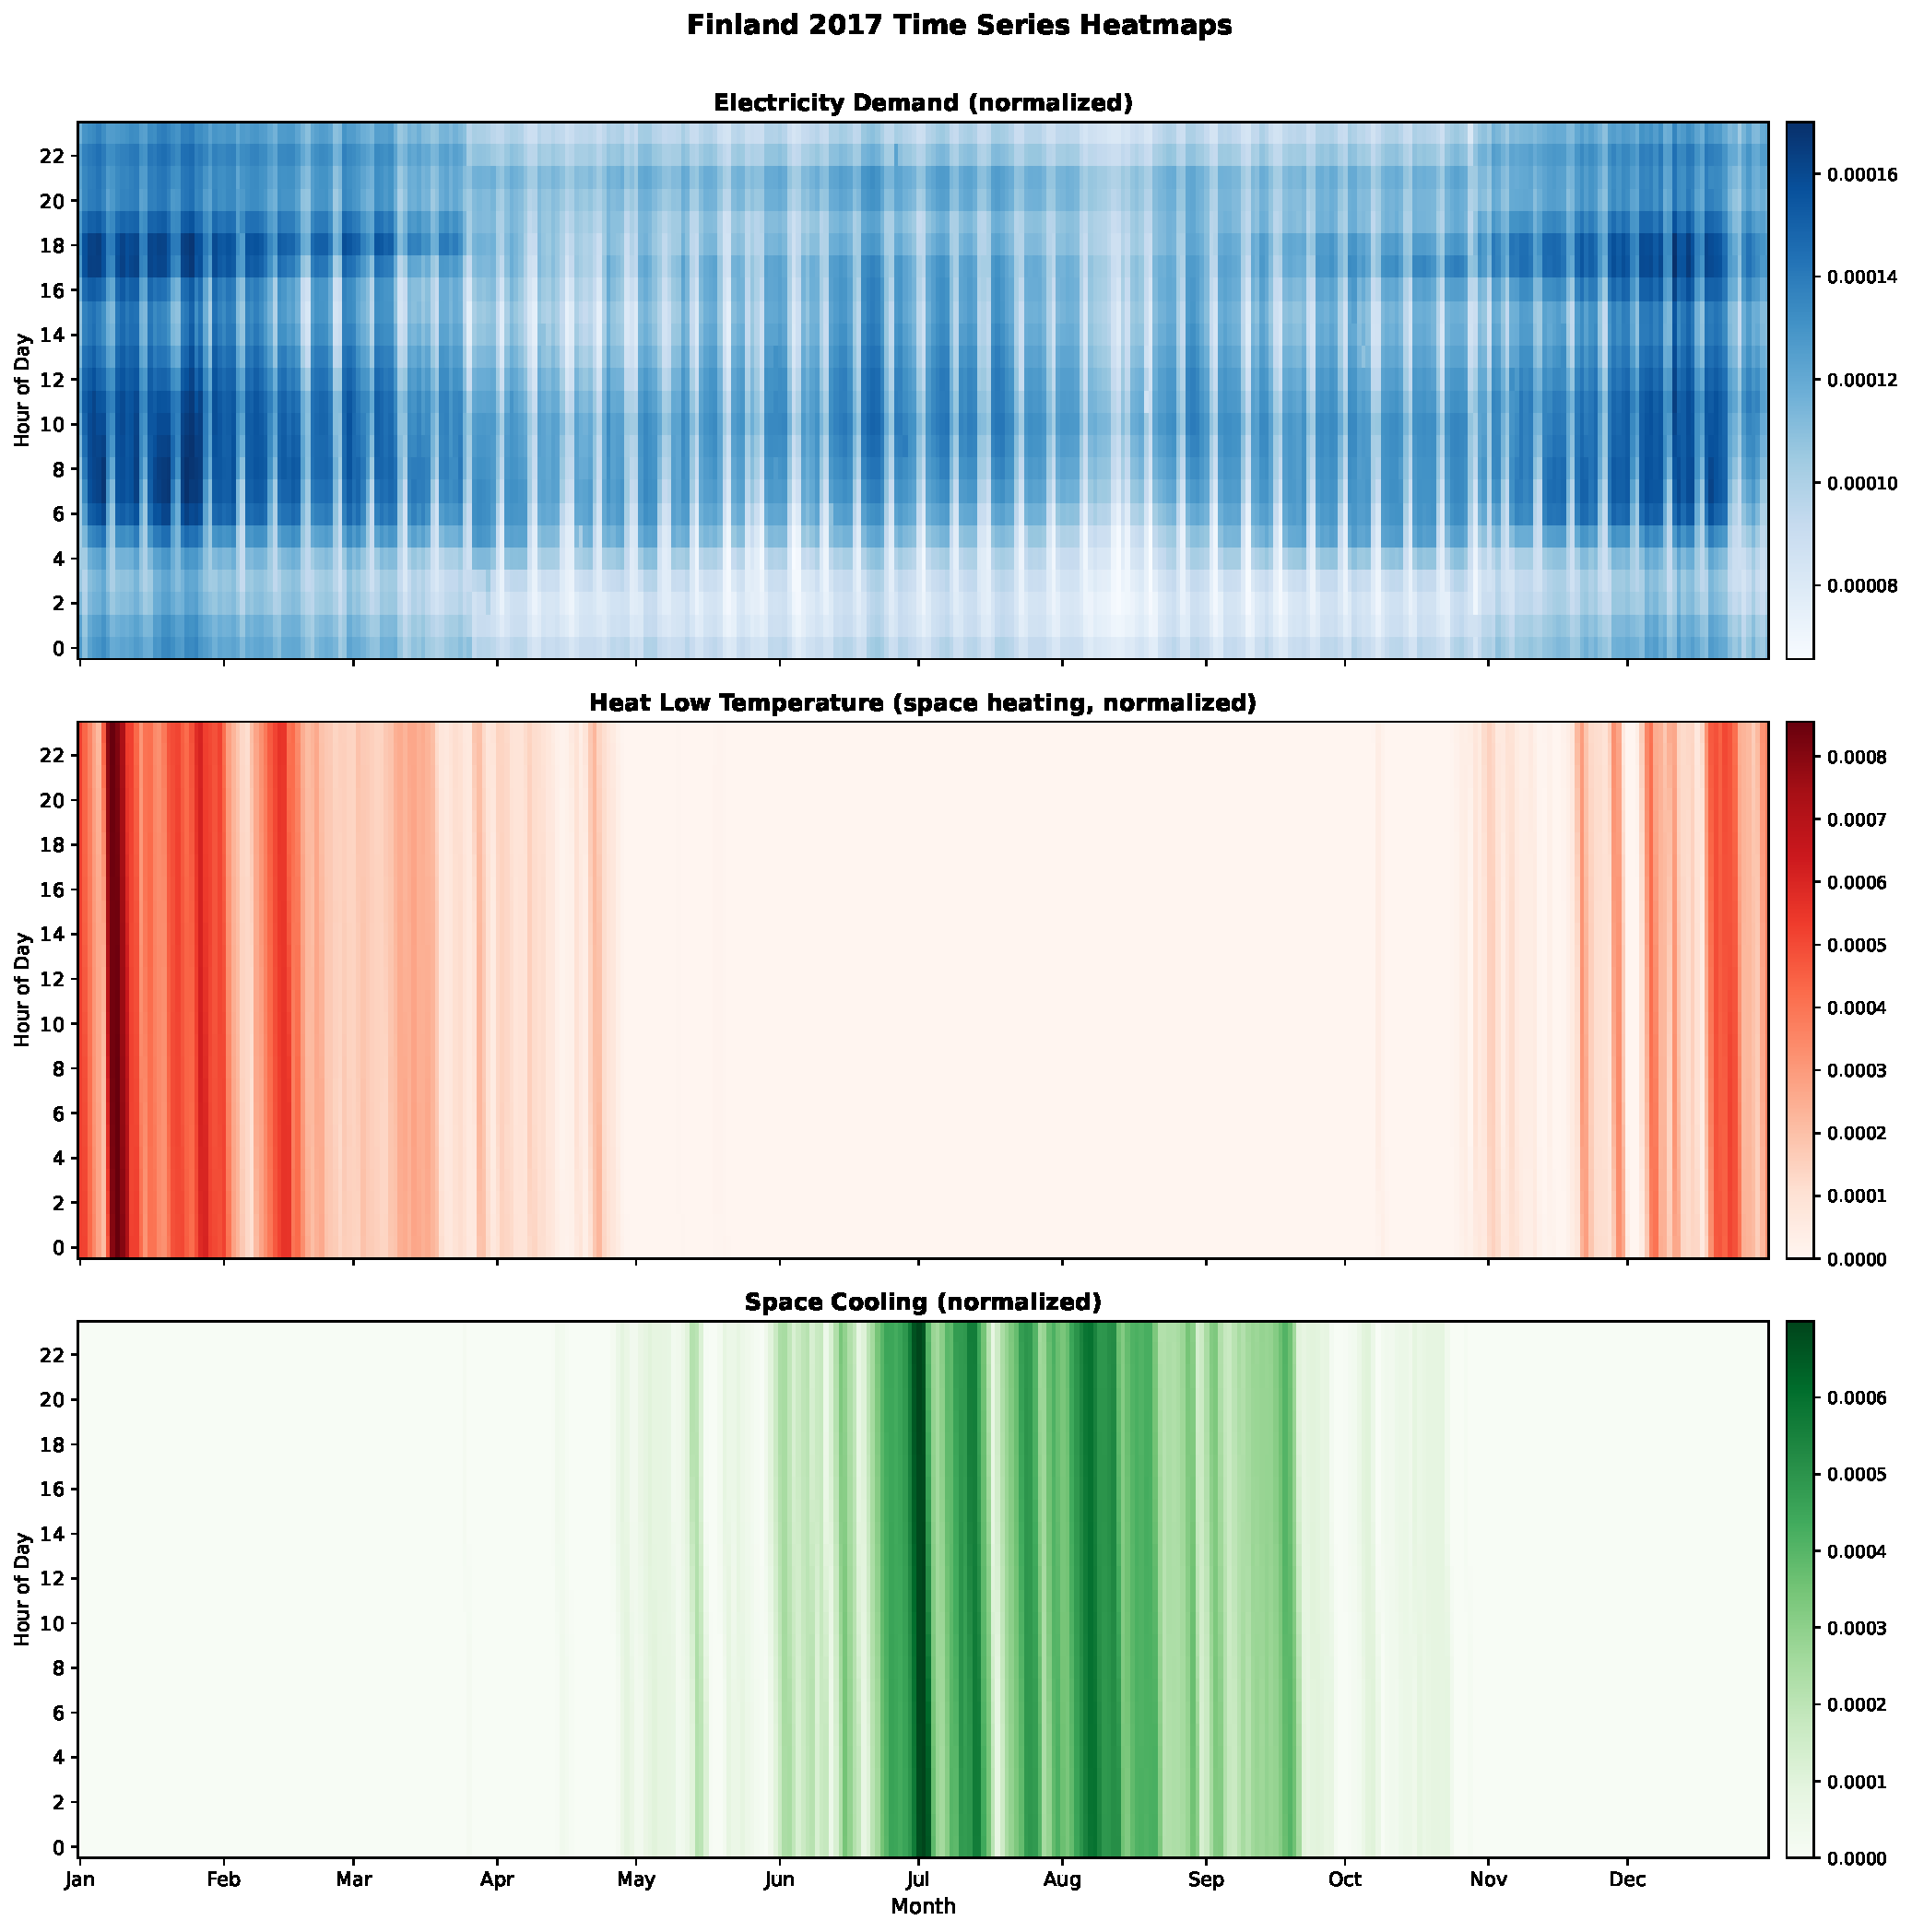
\includegraphics[width=\linewidth]{fi_heatmaps_combined.pdf}
  \caption{Finland (2017, UTC): demand-driver heatmaps used in the typical-day preprocessing. Each panel shows the distribution of hourly demand over the year (normalised profiles), with months on the x-axis and hour of day on the y-axis.}
  \label{fig:fi_td_demand_heatmaps}
\end{figure}

The electricity profile exhibits both intra-day structure (systematic daily cycles) and a marked seasonal component, with higher intensities during the cold season. Low-temperature space-heating demand is strongly seasonal, with a pronounced winter concentration and near-zero levels in summer, reflecting its degree-hour construction. Space-cooling appears as a sparse summer phenomenon, indicating that cooling is a minor driver in the Finnish context and contributes limited discriminatory information outside the warmest weeks. Because all demand series are normalised, the colour intensity should be read as the relative allocation of annual demand across hours rather than absolute load levels.


\begin{figure}[H]
  \centering
  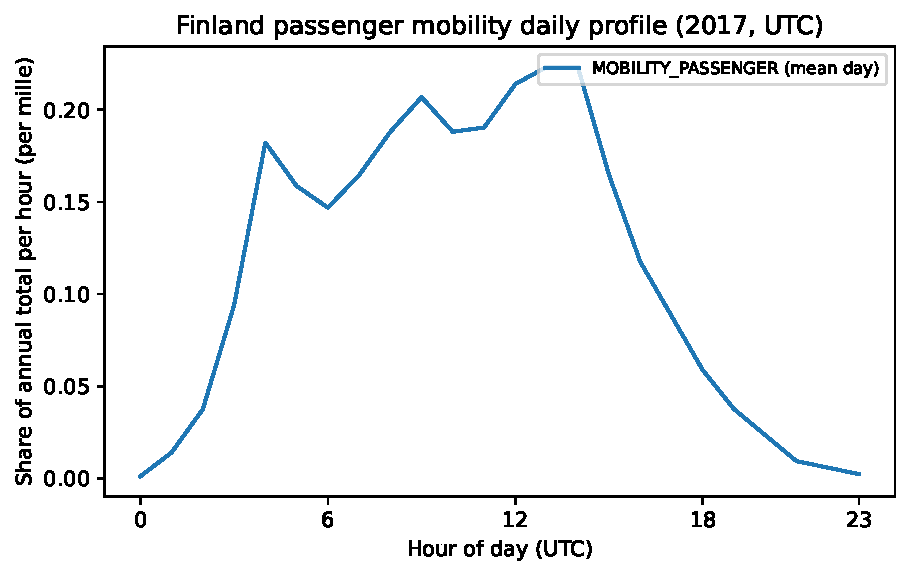
\includegraphics[width=0.78\linewidth]{FI_2017_mobility_passenger_daily_profile.pdf}
  \caption{Passenger mobility daily profile used in EnergyScope Multi-Cells (Finland application, 2017, UTC). The profile is adopted from the EnergyScope TD Belgium setup, itself based on a generic household travel survey hourly pattern, and repeated identically for each day of the year (time-zone mapped).}
  \label{fig:fi_td_mobility_daily}
\end{figure}

The passenger mobility profile is characterised by a morning ramp-up and a broad daytime plateau, followed by a steady decline in the evening. In this modelling framework, the curve is exogenous and does not vary across days, so it does not drive the identification of representative days in clustering. Its role is instead to provide within-day structure for mobility demand once typical days have been selected, ensuring consistent diurnal timing of transport services across scenarios.


\begin{figure}[H]
  \centering
  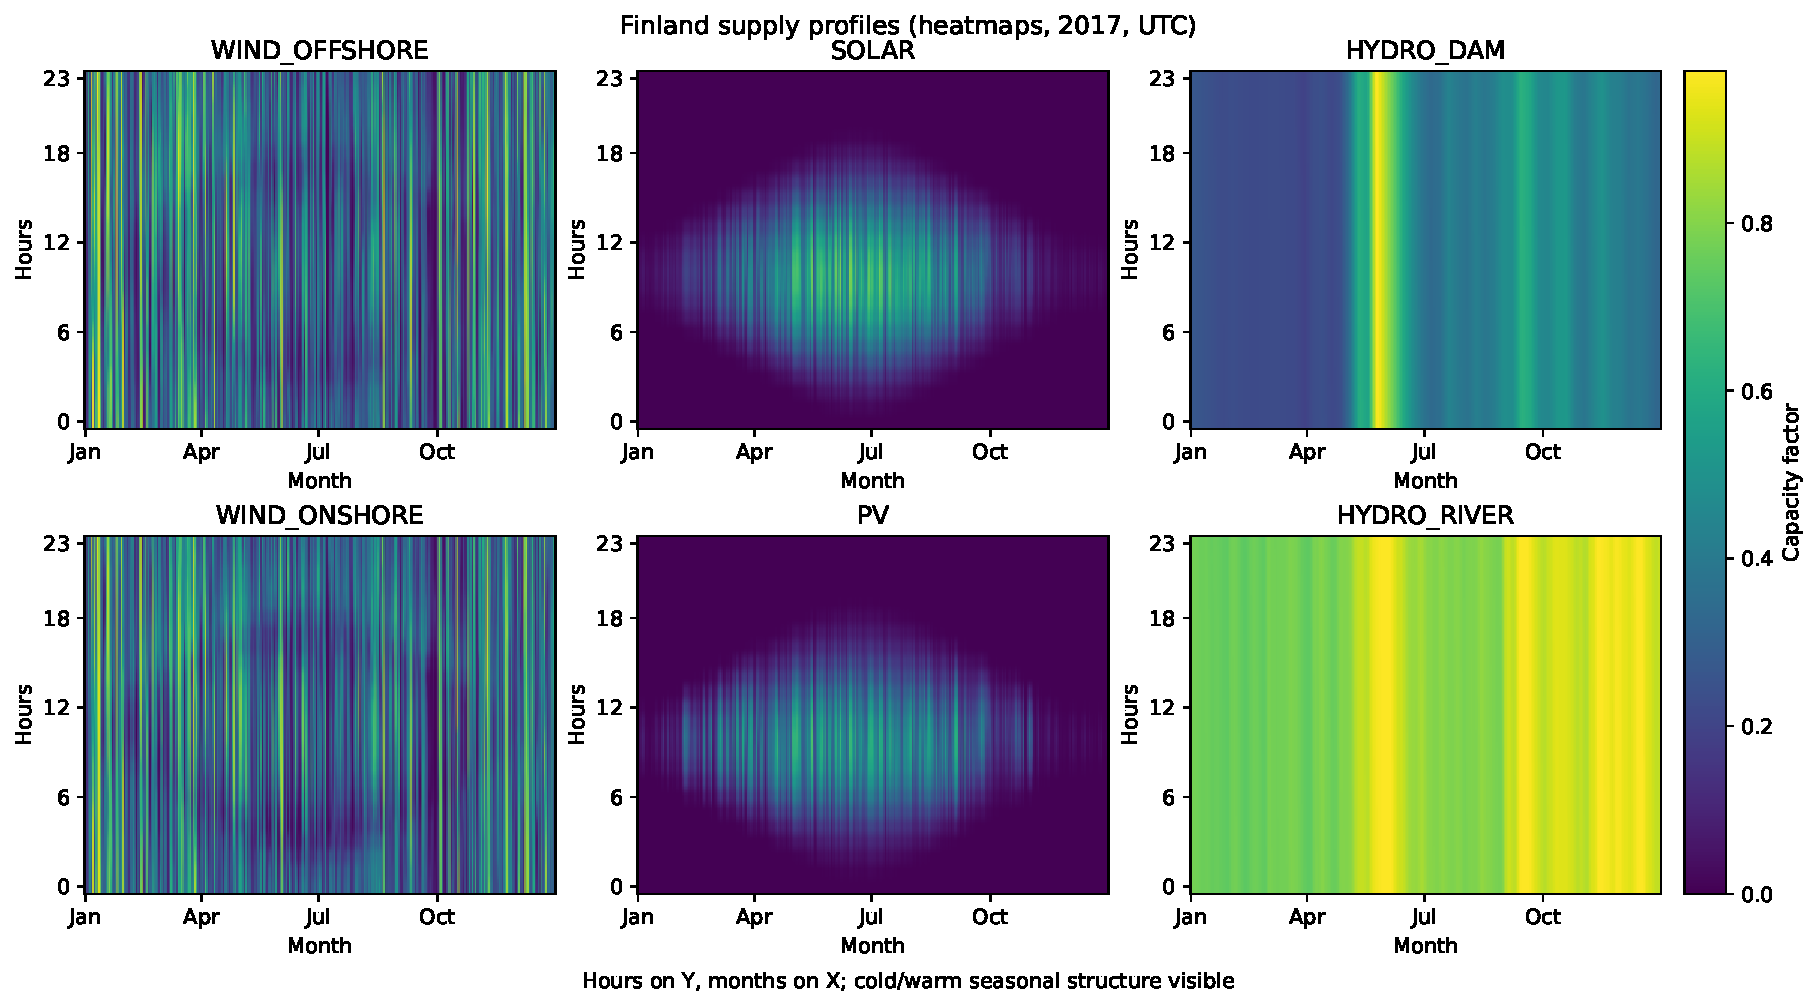
\includegraphics[width=\linewidth]{FI_2017_heatmaps_main.pdf}
  \caption{Finland (2017, UTC): renewable availability heatmaps used as TD inputs. Panels report capacity-factor type hourly profiles for wind (onshore and offshore), solar (thermal proxy) and PV, plus hydropower proxies (dam inflow and run-of-river), and tidal (negligible for Finland, so not plotted)}
  \label{fig:fi_td_renewables_heatmaps}
\end{figure}

Solar and PV exhibit the expected joint diurnal and seasonal structure: near-zero availability during winter and night-time, with sustained daytime generation during summer months. Wind availability shows substantial hour-to-hour and day-to-day variability across the full year, providing strong discriminatory power for typical-day selection. Hydropower proxies are comparatively smoother, with changes that are more seasonal than diurnal, consistent with inflow-driven dynamics and the aggregation procedure used to derive normalised profiles. Together, these patterns motivate including multiple supply-side drivers in the clustering so that typical days reflect both short-term intermittency (wind) and seasonal solar scarcity.

\begin{figure}[H]
  \centering
  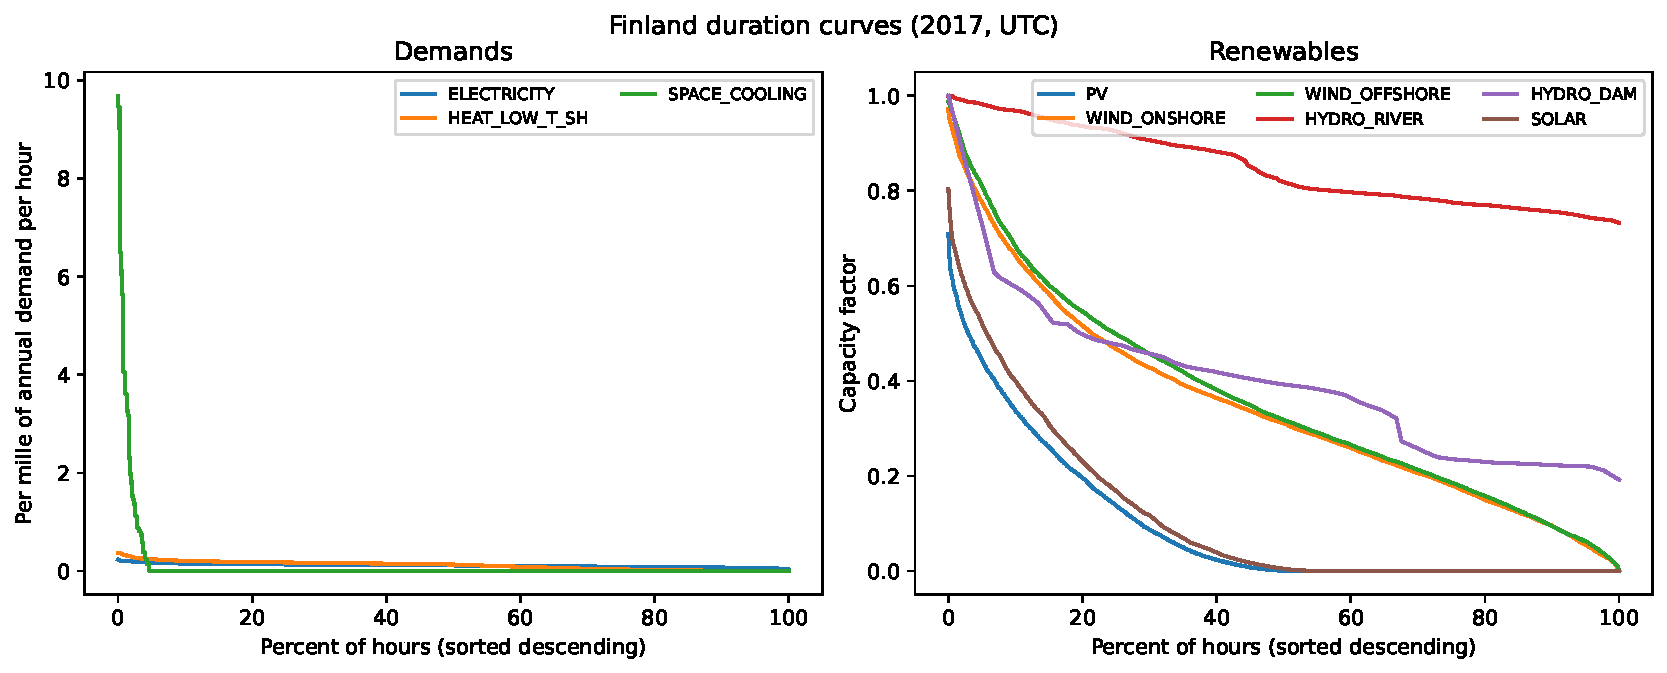
\includegraphics[width=\linewidth]{FI_2017_duration_curves_compact.pdf}
  \caption{Finland (2017, UTC): load duration curves for normalised demand drivers. Curves show the ordered distribution of hourly values (descending), highlighting peakiness and the weight of extreme hours in annual demand profiles.}
  \label{fig:fi_td_duration_curves}
\end{figure}

The electricity duration curve is relatively smooth, indicating that a large portion of annual electricity demand is spread across many hours, with limited reliance on extreme peaks. By contrast, the low-temperature space-heating curve displays a steeper tail, consistent with winter-driven peaks that can materially affect capacity sizing and adequacy constraints. Passenger mobility exhibits a stepped structure because the same diurnal pattern is repeated throughout the year, while freight is flat in the compiled dataset and therefore appears as a constant line. These duration curves provide a compact diagnostic for the extent to which typical days must preserve peak and near-peak hours in order to reproduce sizing-relevant extremes.

As an additional diagnostic, Figure~\ref{fig:fi_td_daily_covariation} reports daily-mean co-variation between selected demand and renewable drivers. While typical-day clustering operates on 24-hour vectors rather than daily averages, these scatter plots clarify cross-variable seasonal structure and motivate retaining multiple drivers in the clustering space.

\begin{figure}[H]
  \centering
  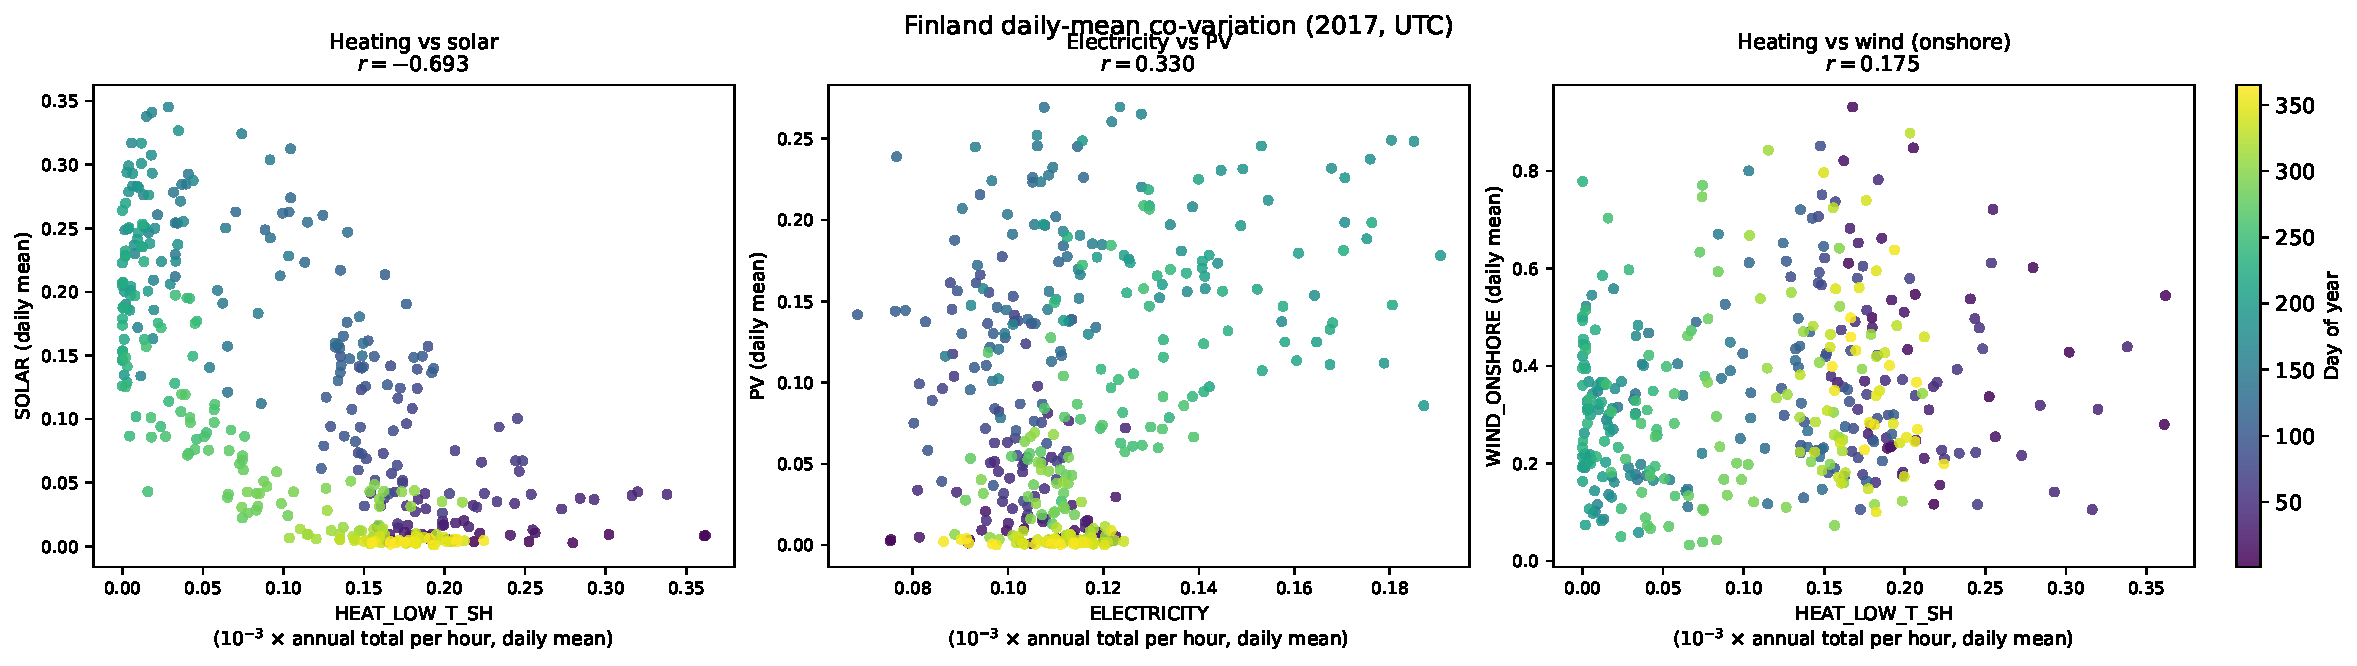
\includegraphics[width=\linewidth]{FI_2017_daily_mean_scatter.pdf}
  \caption{Finland (2017, UTC): daily-mean co-variation between selected TD drivers (colour indicates day of year). Demand variables are shown in per-mille of annual total per hour. Reported $r$ are Pearson correlations across daily means.}
  \label{fig:fi_td_daily_covariation}
\end{figure}


Heating and solar availability are strongly anti-correlated ($r=-0.693$), reflecting a seasonal mismatch in which high space-heating needs coincide with low solar resources. Electricity demand and PV availability display a weaker positive association ($r=0.330$), consistent with both being higher during brighter months while remaining dispersed due to day-to-day weather and non-climatic electricity drivers. Heating and onshore wind show near-independence ($r=0.175$), indicating that wind intermittency is largely orthogonal to heating seasonality; this supports retaining both heating and wind in the feature set so that typical days capture jointly stressful configurations (e.g., cold days with low wind).



In the typical-day construction, we prioritise the most informative drivers of hourly system constraints, namely electricity demand, low-temperature space-heating demand, space-cooling demand (when present), and the main weather-dependent renewable capacity factors (PV and wind, plus run-of-river hydro when available). By contrast, profiles that are flat or nearly invariant across days (for example freight demand in the compiled dataset) provide little discriminatory power for day selection and are therefore not used as primary clustering attributes.

\newpage

\subsubsection{Clustering and representative-day selection}
Let $x_{k,d,h}$ denote the value of time series $k$ at hour $h$ of day $d$. A clustering procedure partitions the $D=365$ days into $N$ clusters, each represented by one TD. In the EnergyScope TD literature, several clustering and representative-day selection strategies are compared, including k-medoids and alternative heuristics; their relative performance depends on the trade-off between computational effort and approximation accuracy \citep{Limpens2021Thesis,ThiranThesis}. The output of this stage is:
(i) a set of TDs,
(ii) a mapping $td(d)$ assigning each original day to a TD, and
(iii) weights $w_{td}$ (the number of original days represented by each TD).

\subsubsection{Chronological reconstruction and storage coupling}
A limitation of TD-based representations is that they can break chronology, which is problematic for storage technologies whose optimal operation depends on sequences of days rather than isolated daily shapes. EnergyScope TD addresses this issue by coupling TD operation with a chronological reconstruction of the year, so that storage state variables evolve over the full horizon while most operational decisions remain defined on the reduced TD set \citep{dominguez-munoz_selection_2011,limpensEnergyScopeTDNovel2019}.

The underlying idea can be understood over a one-week sequence. Calendar days are represented as an ordered list of TD labels (for example, TD~1 on Monday, TD~2 on Tuesday and Wednesday, and TD~3 on weekend days). For a given TD, the intra-day charging and discharging power profile is repeated whenever that TD appears in the sequence, but the stored-energy level is not repeated day by day. Instead, the state of charge is tracked continuously across the entire chronology, linking the end-of-day storage level to the start of the next day even when successive days correspond to different TDs. In practice, this coupling allows the model to exploit TDs to capture typical within-day patterns while still representing inter-day and seasonal storage strategies, such as progressively building reserves across sequences of surplus days and drawing them down during extended deficit periods.

\subsubsection{Optimising the TD set: error metrics and MILP formulation}
EnergyScope TD formalises TD selection using an optimisation-based procedure (MILP) that aims to reduce the approximation error of the reduced time representation. Two complementary error notions are commonly used:
\begin{itemize}
  \item \textbf{Clustering (chronological-shape) error}, measuring how well each day is represented hour-by-hour by its assigned TD.
  \item \textbf{Duration-curve error}, measuring how well the reduced representation reproduces the sorted distribution of hourly values (important for peaks and scarcity periods).
\end{itemize}
A generic formulation (notation adapted from \citet{limpensEnergyScopeTDNovel2019}) is:
\begin{align}
E_{\mathrm{clust}} &= \sum_{k \in \mathcal{K}} \alpha_k \sum_{d=1}^{D} \sum_{h=1}^{24} \left(x_{k,d,h} - \tilde{x}_{k,td(d),h}\right)^2, \\
E_{\mathrm{dc}} &= \sum_{k \in \mathcal{K}} \beta_k \sum_{t=1}^{8760} \left(\mathrm{DC}_k(t) - \widetilde{\mathrm{DC}}_k(t)\right)^2,
\end{align}
where $\mathrm{DC}_k(\cdot)$ is the duration curve (sorted hourly values) of series $k$, and tildes denote the reconstructed values from the TD representation. The MILP chooses the TD set (and assignments) to minimise a weighted combination of these errors subject to selecting exactly $N$ representative days.

Previous EnergyScope TD applications commonly rely on $12$ typical days, which has been identified as a robust compromise between temporal accuracy and computational tractability. In the original EnergyScope TD validation, moving from a full 8{,}760-hour representation to 12 TDs reduces solve times from multi-hour runs to around a minute, making large scenario ensembles and sensitivity analyses feasible. At the same time, 12 TDs were shown to reproduce the full-year ``ground-truth'' solution reasonably well for the main key performance indicators used in planning exercises, including primary energy use, technology capacity choices, total system cost, and aggregate greenhouse-gas emissions. Consistent with this established practice, the present Finland application adopts 12 typical days as a baseline; alternative values can be explored later as a robustness check once the dataset calibration and historical reproduction are consolidated.


\subsection{Step 2: EnergyScope TD optimisation model}

\subsubsection{LP problem: resources, layers, and technologies}
EnergyScope TD represents the energy system as a network of energy \emph{layers} that must be balanced at each time step. Layers include both resources (e.g. natural gas, biomass, solar) and end-use demand layers (e.g. low-temperature heat, passenger mobility), and technologies connect layers through conversion, storage, or infrastructure. Following the EnergyScope terminology, three technology types are distinguished:
(i) end-use type technologies (producing end-use demand layers),
(ii) storage technologies (inter-temporal links within a layer),
and (iii) infrastructure technologies (supporting conversion, networks, and efficiency).

EnergyScope TD is formulated as an LP problem in which the main design variables are installed capacities $F(j)$ for technologies $j$, and the main operational variables are hourly flows (resource uses and technology outputs) defined over hours $h$ and TDs $td$ \citep{limpensGeneratingEnergyTransition2021}. This structure enables rapid solution times that are compatible with extensive scenario sampling. 


The LP solved by EnergyScope TD can be read as a network of balance equations and flow constraints: each coloured \emph{layer} corresponds to an energy-balance equation enforced at every hour (and for each typical day), while each connection corresponds to a non-negative flow variable constrained by technology capacities and conversion coefficients. The solver jointly chooses (i) \emph{design} variables, the installed sizes of assets, and (ii) \emph{operation} variables, the hourly routing of energy through competing pathways to meet end-use demands at minimum system cost. In this network view, storage technologies add inter-temporal coupling by shifting flows across hours, while infrastructure introduces losses and capacity limits, so that the optimum emerges from trading off direct supply, conversion, storage, and cross-sector coupling under resource availability and demand constraints.



\subsubsection{End-use demand in energy services (EUD)}
Following \citet{moret_strategic_2017}, EnergyScope specifies exogenous \emph{end-use demand} (EUD) in terms of energy services rather than \emph{final energy consumption} (FEC). EUD refers to the useful service delivered to end users (e.g., low-temperature heat, passenger-kilometres, ton-kilometres), whereas FEC depends on the chosen conversion pathway and its efficiency. Model inputs are annual sectoral EUD values $endUsesYear(eui,s)$, aggregated into a yearly vector $endUsesInput(eui)$ (Eq.~\eqref{eq:endusesinput}). These yearly totals are then allocated to period-specific demands $EndUses(eut,t)$ through transparent distribution and split rules (Fig.~\ref{fig:enduses_flow}): electricity is distributed uniformly over periods and corrected for grid losses $Loss(Elec,t)$; high-temperature heat is also spread uniformly; low-temperature heat combines space-heating, shaped by an exogenous profile $\%_{\mathrm{sh}}(t)$, with hot-water demand, then splits into district heating and decentralised supply using $\%_{\mathrm{Dhn}}$ (including DHN losses $Loss(HeatLowTDhn,t)$); finally, passenger and freight mobility are distributed uniformly and partitioned by modal shares $\%_{\mathrm{Public}}$ and $\%_{\mathrm{Rail}}$. Consistent with the mapping in Fig.~\ref{fig:enduses_flow}, lighting is not represented as a separate end-use and is instead included in the aggregate electricity end-use. The allocation and split parameters (e.g., $\%_{\mathrm{Public}}$, $\%_{\mathrm{Rail}}$, $\%_{\mathrm{Dhn}}$, and the space-heating profile $\%_{\mathrm{sh}}(t)$) are country-specific, as they reflect national patterns in modal shares, heating infrastructures, and seasonal demand. In the Finnish application, these parameters therefore need to be calibrated to Finland using national energy and transport statistics to ensure that the mapping from $endUsesInput$ to $EndUses(eut,t)$ matches observed end-use structures (see Table \ref{tab:fin_eud_params_2020}).


The monthly totals obtained by summing the compiled hourly profiles provide a simple diagnostic of how yearly end-use demand is allocated across the calendar. Because each series is normalised over the year, monthly sums should be read as shares of the annual end-use rather than as absolute energy levels. In the Finnish case, this diagnostic confirms the strong winter concentration of low-temperature space-heating demand, whereas electricity remains comparatively flatter across months and passenger mobility remains close to uniform because its diurnal shape is repeated throughout the year in the compiled dataset. This seasonality check helps identify which end-uses provide the strongest temporal signal that the typical-day selection must preserve.



\begin{figure}[t]
\centering
\resizebox{0.98\linewidth}{!}{%
\begin{tikzpicture}[
  font=\small,
  flow/.style={line width=0.6pt, line cap=round},
  lblL/.style={anchor=east, align=left},
  lblR/.style={anchor=west, align=left},
  lab/.style={font=\scriptsize, inner sep=1pt, fill=white},
  sum/.style={circle, draw, line width=0.6pt, inner sep=1.3pt}
]

\def\xLabelL{0.0}
\def\xStart{1.2}
\def\xJoin{8.0}
\def\xSplit{10.2}
\def\xEnd{15.2}
\def\xLabelR{16.1}

\def\yElec{5.0}
\def\yHT{3.9}
\def\ySH{2.6}
\def\yHW{1.7}
\def\yPass{0.4}
\def\yFre{-0.7}

\def\yDHN{2.9}
\def\yDec{2.1}
\def\yPub{0.8}
\def\yPriv{0.0}
\def\yRail{-0.4}
\def\yRoad{-1.2}

% ------------------------
% Headings (fixed, no overlap)
% ------------------------
\node[anchor=south west] at (\xStart,\yElec+1.05)
{$endUsesInput(eui)=\sum_{s\in S} endUsesYear(eui,s)\qquad \forall eui\in EUI$};

\node[anchor=south east] at (\xEnd,\yElec+1.05)
{$EndUses(eut,t)$};

% Left labels
\node[lblL] at (\xLabelL,\yElec) {ELECTRICITY};
\node[lblL] at (\xLabelL,\yHT)   {HEAT HIGH T};
\node[lblL] at (\xLabelL,\ySH)   {HEAT LOW T (SH)};
\node[lblL] at (\xLabelL,\yHW)   {HEAT LOW T (HW)};
\node[lblL] at (\xLabelL,\yPass) {MOB.\ PASSENGER};
\node[lblL] at (\xLabelL,\yFre)  {MOB.\ FREIGHT};

% Right labels
\node[lblR] at (\xLabelR,\yElec) {ELECTRICITY};
\node[lblR] at (\xLabelR,\yHT)   {HEAT HIGH T};
\node[lblR] at (\xLabelR,\yDHN)  {HEAT LOW T DHN};
\node[lblR] at (\xLabelR,\yDec)  {HEAT LOW T DECEN};
\node[lblR] at (\xLabelR,\yPub)  {MOB.\ PUBLIC};
\node[lblR] at (\xLabelR,\yPriv) {MOB.\ PRIVATE};
\node[lblR] at (\xLabelR,\yRail) {MOB.\ FREIGHT RAIL};
\node[lblR] at (\xLabelR,\yRoad) {MOB.\ FREIGHT ROAD};

% Electricity (lighting omitted)
\draw[flow] (\xStart,\yElec) -- (\xEnd,\yElec)
  node[lab, pos=0.46, above=2pt] {$\cdot \dfrac{1}{\sum_{t'\in T} t_{op}(t')}$}
  node[lab, pos=0.74, above=2pt] {$+\,Loss(Elec,t)$};

% Heat high T
\draw[flow] (\xStart,\yHT) -- (\xEnd,\yHT)
  node[lab, pos=0.46, above=2pt] {$\cdot \dfrac{1}{\sum_{t'\in T} t_{op}(t')}$};

% Low-T heat: SH + HW then split
\node[sum] (sumHeat) at (\xJoin,2.15) {$+$};

\draw[flow] (\xStart,\ySH) -- (\xJoin-1.6,\ySH)
  node[lab, pos=0.55, above=2pt] {$\cdot \dfrac{\%_{\mathrm{sh}}(t)}{t_{op}(t)}$}
  -- (\xJoin-1.6,2.15) -- (sumHeat.west);

\draw[flow] (\xStart,\yHW) -- (\xJoin-1.6,\yHW)
  node[lab, pos=0.55, below=2pt] {$\cdot \dfrac{1}{\sum_{t'\in T} t_{op}(t')}$}
  -- (\xJoin-1.6,2.15) -- (sumHeat.west);

\coordinate (heatSplit) at (\xSplit,2.15);
\draw[flow] (sumHeat.east) -- (heatSplit);

\draw[flow] (heatSplit) -- (\xEnd,\yDHN)
  node[lab, pos=0.56, above=2pt] {$\cdot \%_{\mathrm{Dhn}} \;+\; Loss(HeatLowTDhn,t)$};

\draw[flow] (heatSplit) -- (\xEnd,\yDec)
  node[lab, pos=0.56, below=2pt] {$\cdot (1-\%_{\mathrm{Dhn}})$};

% Passenger mobility split
\coordinate (passSplit) at (\xSplit,\yPass);
\draw[flow] (\xStart,\yPass) -- (passSplit)
  node[lab, pos=0.52, above=2pt] {$\cdot \dfrac{1}{\sum_{t'\in T} t_{op}(t')}$};

\draw[flow] (passSplit) -- (\xEnd,\yPub)
  node[lab, pos=0.56, above=2pt] {$\cdot \%_{\mathrm{Public}}$};

\draw[flow] (passSplit) -- (\xEnd,\yPriv)
  node[lab, pos=0.56, below=2pt] {$\cdot (1-\%_{\mathrm{Public}})$};

% Freight mobility split
\coordinate (freSplit) at (\xSplit,\yFre);
\draw[flow] (\xStart,\yFre) -- (freSplit)
  node[lab, pos=0.52, above=2pt] {$\cdot \dfrac{1}{\sum_{t'\in T} t_{op}(t')}$};

\draw[flow] (freSplit) -- (\xEnd,\yRail)
  node[lab, pos=0.56, above=2pt] {$\cdot \%_{\mathrm{Rail}}$};

\draw[flow] (freSplit) -- (\xEnd,\yRoad)
  node[lab, pos=0.56, below=2pt] {$\cdot (1-\%_{\mathrm{Rail}})$};

\end{tikzpicture}%
}
\caption{Mapping from yearly end-use inputs $endUsesInput$ to period-specific demands $EndUses(eut,t)$, with lighting aggregated into the electricity end-use. Adapted from \citet{moret_strategic_2017}.}
\label{fig:enduses_flow}
\end{figure}

\begin{table}[h!]
\footnotesize
\centering
\begin{threeparttable}
\caption{Finland calibration targets for the EUD mapping (baseline year 2020).}
\label{tab:fin_eud_params_2020}

% Choose a width for the Source column that fits your page.
% Here: last column wraps at ~55% of linewidth.
\begin{tabular}{@{} l l l >{\raggedright\arraybackslash}p{0.35\linewidth} @{}}
\toprule
Parameter & Symbol & Value & Source \\
\midrule
District heating share of low-T heat\tnote{a} &
$\%_{\mathrm{Dhn}}$ &
0.45 &
\href{https://energia.fi/wp-content/uploads/2024/01/Energy-Year-2023_DistrictHeating.pdf}{Finnish Energy (2024)} \\

District heating network losses\tnote{b} &
$Loss(\mathrm{HeatLowTDhn})$ &
0.085 &
\href{https://energia.fi/en/energy-sector-in-finland/energy-networks/district-heating-networks/}{Finnish Energy (2024)} \\

Inland public passenger mobility share\tnote{c} &
$\%_{\mathrm{Public}}$ &
0.1608 &
\href{https://stat.fi/til/tiet/2019/tiet_2019_2020-04-15_en.pdf}{Statistics Finland (2020), \emph{Traffic on highways 2019}}
; \href{https://stat.fi/til/rtie/2019/rtie_2019_2020-08-27_en.pdf}{Statistics Finland (2020), \emph{Railway statistics 2019}} \\

Inland rail freight share\tnote{d} &
$\%_{\mathrm{Rail}}$ &
0.2761 &
\href{https://stat.fi/til/rtie/2019/rtie_2019_2020-08-27_en.pdf}{Statistics Finland (2020), \emph{Railway statistics 2019}}
; \href{https://stat.fi/til/kttav/2019/kttav_2019_2020-04-28_en.pdf}{Statistics Finland (2020), \emph{Goods transport by road 2019}} \\

Electricity grid losses\tnote{e} &
$Loss(\mathrm{Elec})$ &
0.03 &
\href{https://www.doria.fi/bitstream/10024/185778/1/yene_efp_202200_2022_25869_net.pdf}{Finnish Energy and Statistics Finland (2022), \emph{Energy in Finland 2022}} \\
\bottomrule
\end{tabular}

\begin{tablenotes}\footnotesize
\item[a] Proxy for the DHN split: district heating share of heating energy / space-heating market in Finland (year 2020).
\item[b] Implemented as a constant loss factor; Finnish Energy reports typical DH distribution losses of 8--9\% of transmitted energy, hence 0.085 as midpoint.
\item[c] Computed as $(\mathrm{pkm}_{\mathrm{bus}}+\mathrm{pkm}_{\mathrm{rail}})/(\mathrm{pkm}_{\mathrm{car}}+\mathrm{pkm}_{\mathrm{bus}}+\mathrm{pkm}_{\mathrm{rail}})$ using pre-COVID 2019 inland passenger-km: $\mathrm{pkm}_{\mathrm{car}}=66.8$ bn and $\mathrm{pkm}_{\mathrm{bus}}=7.9$ bn (\emph{Traffic on highways 2019}), and $\mathrm{pkm}_{\mathrm{rail}}=4.9$ bn (\emph{Railway statistics 2019}). 2019 is used as a structural proxy to avoid pandemic-related distortions in 2020 modal shares.
\item[d] Computed as $\mathrm{tkm}_{\mathrm{rail}}/(\mathrm{tkm}_{\mathrm{rail}}+\mathrm{tkm}_{\mathrm{road}})$ using pre-COVID 2019 inland freight tonne-km: $\mathrm{tkm}_{\mathrm{rail}}=10.3$ bn (\emph{Railway statistics 2019}) and $\mathrm{tkm}_{\mathrm{road}}\approx 27.0$ bn from domestic road freight performance reported as ``close on 27 million tonne-kilometres'' in \emph{Goods transport by road 2019} (interpreted as 27,000 million tonne-km).
\item[e] Electricity transmission and distribution losses are set to 0.03 based on the ``Losses 3\%'' entry reported in the electricity consumption breakdown in \emph{Energy in Finland 2022} (compiled from Finnish Energy and Statistics Finland). Used as a constant proxy for baseline year 2020.
\end{tablenotes}
\end{threeparttable}
\end{table}





\subsubsection{Objective function: total annual cost (and emissions accounting)}
A standard objective is the minimisation of total annualised system cost,
decomposed into annualised investment costs, fixed operation and maintenance costs, and resource operating costs \citep{limpensEnergyScopeTDNovel2019}:
\begin{align}
\min \; C_{\mathrm{tot}}
= \sum_{j \in \mathcal{TECH}} \left[\tau(j)\, C_{\mathrm{inv}}(j) + C_{\mathrm{maint}}(j)\right]
+ \sum_{i \in \mathcal{RES}} C_{\mathrm{op}}(i),
\end{align}
with $\tau(j)$ an annualisation factor that depends on the discount rate and lifetime. 
In addition, annual system-wide GHG emissions are computed with a life cycle assessment approach, accounting for “cradle-to-grave” emissions from both technologies and energy resources. Climate impacts are reported using global warming potential (GWP) in ktCO\textsubscript{2}-eq per year. Total yearly emissions, $GWP_{\text{tot}}$ (Eq.~\eqref{eq:gwp_total}), are defined as the sum of (i) the construction and end-of-life impacts of energy conversion technologies, annualised by their lifetime, and (ii) operational impacts from resources, including fuel supply chains (up to combustion) and imported electricity, weighted by the operating period.

Following \citet{limpensEnergyScopeTDNovel2019}:

\begin{equation}
GWP_{\mathrm{tot}} \;=\; \sum_{j \in \mathrm{TECH}} \frac{GWP_{\mathrm{constr}}(j)}{\mathrm{lifetime}(j)} \;+\; \sum_{i \in \mathrm{RES}} GWP_{\mathrm{op}}(i)
\label{eq:gwp_total}
\end{equation}
 


\subsubsection{Seasonality and long-term storage: coupling typical days}
A known limitation of TD approaches is the difficulty to represent inter-day dynamics and seasonal storage. EnergyScope TD implements a reconstruction method in which each day of the year is assigned to a TD through a sequence, while the stored-energy state variable is tracked across all 8760 hours. Operational variables other than stored energy remain defined on the TD basis \citep{limpensGeneratingEnergyTransition2021}. This enables modelling of day-to-day and seasonal storage strategies without solving the full hourly year.

Because EnergyScope TD is designed for fast whole-system optimisation, it abstracts from some short-term operational details (e.g. unit commitment or detailed ramping constraints) that are central in dispatch-focused models. The TD approach is therefore best interpreted as a planning-level representation that trades operational detail for tractability, and can be complemented by more detailed operational checks when needed \citep{thiranExploringOptionsFossilfree2025}.


% ------------------------------------------------------------------
\subsubsection{Biomass modelling: feedstocks, supply curves, and Finland-specific calibration}
\label{sec:biomass_modelling}

\paragraph{Why biomass calibration is a first-order modelling choice.}
Bioenergy potentials are not uniquely defined objects: reported values differ widely because they embed distinct assumptions about sustainability constraints, competing uses (materials, soil functions, circularity), land allocation for energy crops, and waste management pathways. Selecting a given ``potential'' is therefore a structural modelling choice that shapes the socio-technical system being represented. \citet{collaNavigatingBioenergyHorizons2024} illustrate this point by showing that European assessments can imply markedly different 2030 bioenergy ranges for a single country (Belgium: 30--90~TWh across four studies), with divergences driven primarily by (i) how competing uses are accounted for, (ii) land-use rules for energy crops, and (iii) whether waste streams are directed to energy or material recovery. At the European scale, they argue that a ``realistic'' order of magnitude for EU27+UK in 2030 lies in the lower part of published ranges (about 2000--2500~TWh), noting that forestry feedstocks are already relatively exploited while additional mobilisation would come mainly from agricultural residues, conditional on collection practices and farm structure \citep{collaNavigatingBioenergyHorizons2024}. These lessons motivate a transparent, scenario-based calibration strategy for Finland rather than reliance on a single headline potential.

\paragraph{Stage 1: what is transferred from the Belgian EnergyScope implementation.}
The Belgian application of \citet{collaOptimalUseLignocellulosic2022} presents lignocellulosic biomass through cost supply curves, an origin-by-quality decomposition, and step-specific embedded GHG intensities. Their Belgium case therefore makes three modelling choices explicit: biomass is procured in merit order, different fractions have different marginal costs, and different fractions carry different supply-chain carbon footprints. We retain that logic in the Finnish first stage because it is the right level of detail for asking where a scarce biomass resource is most valuable once system-wide GHG constraints bind.

\paragraph{First-stage simplification for Finland.}
The current Finnish implementation does not reproduce the full Belgian origin-by-quality matrix. Instead, it collapses the forest-biomass ladder into four domestic steps and one import backstop. This is a deliberate simplification because the present paper studies forest-management intensity and biodiversity constraints in Finland, not the full geography of European biomass trade. Four simplifications should therefore be stated explicitly:
\begin{enumerate}
  \item The domestic ladder aggregates the Finnish forest resource into industrial by-products, logging residues, secondary woodchips/sawdust, and direct fuelwood/landscape wood, rather than distinguishing all Belgian origin rings and quality classes separately.
  \item Step-specific embedded GHG coefficients are retained, but they are implemented as pragmatic first-stage supply-chain coefficients attached to the Finnish steps, not as a full re-estimation of every RED~II category used in the Belgian case.
  \item The Belgian low-quality share constraint is not re-implemented at this stage. The Finnish first-stage model therefore captures relative cost and relative GHG differences between steps, but not a separate ash-content or quality-mixing constraint.
  \item The Finnish scenarios are parameterised to represent forest-policy narratives, not to claim direct measurement of future biomass availability. In particular, S1/BES is stylised and S3/BDS is a conservative audited scenario rather than a raw database value.
\end{enumerate}

\paragraph{Supply curves in the linear programme.}
Let $r \in \{\text{WOOD\_FI1},\dots,\text{WOOD\_FI5}\}$ denote a Finnish biomass step. We introduce decision variables $x_r$ (annual energy procured from step $r$), with exogenous step capacities $\overline{X}_r$, marginal supply costs $c_r$, and embedded supply-chain GHG intensities $g_r$. The first-stage formulation is:
\begin{align}
0 \leq x_r &\leq \overline{X}_r \qquad \forall r,
\label{eq:bio_segment_cap}\\
C_{\text{bio}} &= \sum_r c_r\,x_r,
\label{eq:bio_cost}\\
\text{GHG}_{\text{bio,supply}} &= \sum_r g_r\,x_r.
\label{eq:bio_ghg}
\end{align}
This formulation preserves the key logic of the Belgian approach: the optimiser first uses the cheapest domestic fractions and only reaches the high-cost import backstop when cheaper Finnish steps are exhausted.

\begin{figure}[t]
\centering
% Shift slightly left and scale down to fit the page without overflow.
\makebox[\linewidth][c]{\hspace*{-0.55cm}\begin{tikzpicture}[
  font=\small,
  scale=0.95, transform shape,
  box/.style={draw, rounded corners, align=center, inner sep=6pt},
  sbox/.style={draw, rounded corners, align=left, inner sep=6pt},
  arr/.style={-Latex, thick},
  faint/.style={draw, rounded corners, dashed, inner sep=8pt}
]

% Left block: potentials and scenario levers
\node[box, text width=4.1cm] (pot) {\textbf{Woody biomass potentials}\\
\footnotesize Domestic + imports, represented as supply curves};

\node[sbox, below=3mm of pot, text width=4.1cm] (lev) {\textbf{Scenario levers (Stage 2)}\\
\footnotesize
Policy regimes (biodiversity, sinks)\\
Physical-risk shocks (storm, fire, pests)\\
Market shocks (prices, import frictions)\\
\(\Rightarrow\) modify \(\overline{X}_{b,o,q,s}\), \(c_{b,o,q,s}\)};

\node[sbox, below=3mm of lev, text width=4.1cm] (qual) {\textbf{Feedstock structure (Stage 1)}\\
\footnotesize
Origin rings (domestic, neighbour, EU, RoW)\\
Quality classes (good vs low)\\
Quality-share constraint \(\alpha_{\mathrm{low}}\)\\
Embedded GHG factors \(g_{b,o,q}\)};

\node[faint, fit=(pot)(lev)(qual)] (leftfit) {};

% Middle block: technology portfolio (baseline)
\node[box, right=10mm of pot, text width=4.3cm] (tech) {\textbf{Conversion portfolio}\\
\footnotesize Stage 1: adopt Colla framework};

\node[sbox, below=3mm of tech, text width=4.3cm] (techlist) {\textbf{Route families (synthetic)}\\
\footnotesize
Direct heat: boilers (LT, DH, industrial)\\
CHP: heat + power (DH and industry)\\
Dispatchable biomass power\\
Thermochemical gas: gasification \(\rightarrow\) SNG\\
Thermochemical liquids: SLF (e.g.\ FT-type)\\
Optional upgrading and conditioning};

\node[sbox, below=3mm of techlist, text width=4.3cm] (techpar) {\textbf{Key techno-economic inputs}\\
\footnotesize
Efficiencies and co-products\\
CAPEX, OPEX, lifetimes\\
Operating constraints\\
Compatibility with quality classes};

\node[faint, fit=(tech)(techlist)(techpar)] (midfit) {};

% Right block: end uses and system constraints
\node[box, right=10mm of tech, text width=4.3cm] (end) {\textbf{Competing end uses}\\
\footnotesize Allocation decided endogenously};

\node[sbox, below=3mm of end, text width=4.3cm] (endlist) {\textbf{Final needs served}\\
\footnotesize
Low-temperature heat (buildings)\\
District heating and medium-T heat\\
High-temperature industrial heat\\
Electricity (dispatchable)\\
Mobility fuels (where relevant)\\
Non-energy demand (feedstocks)};

\node[sbox, below=3mm of endlist, text width=4.3cm] (sys) {\textbf{System drivers (common)}\\
\footnotesize
GHG cap and accounting\\
Energy service demands (EUD)\\
Competing low-carbon options\\
Shadow prices reveal scarcity};

\node[faint, fit=(end)(endlist)(sys)] (rightfit) {};

% Arrows
\draw[arr] (leftfit.east) -- node[above, font=\footnotesize] {supply curves} (midfit.west);
\draw[arr] (midfit.east) -- node[above, font=\footnotesize] {energy carriers} (rightfit.west);

% Optional feedback (dashed)
\draw[-Latex, dashed] (sys.west) .. controls ($(sys.west)+(-1.0,0.8)$) and ($(techpar.east)+(1.0,0.8)$) .. (techpar.east);

\end{tikzpicture}}%
\caption{Structure of the woody-biomass module in EnergyScope TD. Stage 1 reproduces the biomass modelling base of Colla et al.\ (conversion portfolio, costs, and import segmentation) to ensure internal consistency and comparability. Stage 2 introduces Finland-specific biomass potential narratives by shifting supply-curve segment capacities and marginal costs, thereby testing how the optimisation reallocates biomass across competing end uses under a binding GHG cap.}
\label{fig:biomass_module_structure}
\end{figure}

\paragraph{Reading Figure~\ref{fig:biomass_module_structure}.}
Biomass ``potential'' enters the optimisation through supply curves, so policy constraints and physical-risk narratives translate into explicit shifts in availability (\(\overline{X}_{b,o,q,s}\)) and delivered costs (\(c_{b,o,q,s}\)), rather than a single exogenous scalar. Given a conversion portfolio (Stage 1 baseline), the model allocates lignocellulosic biomass endogenously across final needs under system-wide constraints. In stringent GHG settings, shadow prices and selected routes indicate where biomass becomes most valuable and which end uses are crowded out first when availability is tightened or prices increase.

\paragraph{Biomass conversion technologies and allocation across end uses.}
The Stage 1 conversion portfolio (Figure~\ref{fig:biomass_module_structure}, middle block) is designed to represent the main lignocellulosic routes competing in deep decarbonisation contexts, including direct heat and CHP options as well as thermochemical pathways producing gaseous or liquid fuels that can serve high-temperature applications and non-energy demand \citep{collaOptimalUseLignocellulosic2022}. This whole-system competition is essential for identifying when biomass is used as a bulk energy source versus when it is reserved for end uses with fewer low-carbon substitutes.

\paragraph{Verified sources for the Finnish supply ladder.}
The neutral reference case S2/NFS is built from the ENSPRESO medium potential for Finland, interpolated to 2035 at the commodity-code level before aggregation into the four domestic steps \citep{ruizENSPRESOOpenEU282019}. The stylised S1/BES case is then constructed as a +20\% scale-up of the S2 ladder. This is not presented as a literal replication of the BES harvest simulated by Blattert et al.; it is a sensitivity case used because the ENSPRESO high scenario for Finland yields implausibly large forest-energy volumes and because the BES narrative increases some residue streams without simply increasing all wood categories proportionally \citep{blattertSectoralPoliciesCause2022}. Importantly, \citet{blattertSectoralPoliciesCause2022} find that BES achieves only 75\% of the maximum possible harvest when biodiversity non-decline is simultaneously enforced, and that higher residue mobilisation roughly offsets lower roundwood, so that BES produces approximately equivalent total wood energy to NFS; the +20\% parameterisation is therefore a deliberate high-biomass sensitivity bound rather than a scenario-faithful reconstruction of the simulated BES outcomes. The conservative S3/BDS case is not the original ENSPRESO low value of 74.2~TWh. That initial value was revised downward after a three-way audit combining the biodiversity-constrained forest-management narrative of Blattert et al., the ecological harvest ceiling proposed by M\"onkk\"onen et al., and a cross-check against recent Finnish national wood-energy statistics \citep{blattertSectoralPoliciesCause2022,monkkonenEcologicallyEconomicallySustainable2024,lukeWoodEnergy2024}. The revised domestic S3 ceiling is 40~TWh, split across the four domestic steps as 32.0, 6.0, 1.5, and 0.5~TWh.

\begin{table}[t]
\centering
\footnotesize
\caption{First-stage Finnish forest-biomass ladder used in the 2035 scenarios. Embedded GHG covers harvesting, preprocessing, and transport only; it does not represent biogenic combustion CO$_2$.}
\label{tab:fi_biomass_ladder}
\begin{tabularx}{\linewidth}{>{\raggedright\arraybackslash}p{2.2cm}X>{\centering\arraybackslash}p{2.2cm}>{\centering\arraybackslash}p{2.3cm}}
\toprule
\textbf{Step} & \textbf{Interpretation and main source mapping} & \textbf{Cost} & \textbf{Embedded GHG} \\
 &  & \textbf{(€/MWh)} & \textbf{(tCO$_2$eq/GWh)} \\
\midrule
\texttt{WOOD\_FI1} & Industrial by-products from chemical and physical wood processing, primarily black liquor, bark, and sawdust (ENSPRESO \texttt{MINBIOWOOa}) & 11 & 20 \\
\texttt{WOOD\_FI2} & Logging residues such as branches and tops (ENSPRESO \texttt{MINBIOFRSR1}) & 22 in S1/S2; 26 in S3 & 22 \\
\texttt{WOOD\_FI3} & Secondary woodchips and sawdust streams (ENSPRESO \texttt{MINBIOWOOW1} + \texttt{MINBIOWOOW1a}) & 27 & 24 \\
\texttt{WOOD\_FI4} & Direct fuelwood and landscape-care wood (ENSPRESO \texttt{MINBIOWOO} + \texttt{MINBIOFRSR1a}) & 33 & 26 \\
\texttt{WOOD\_FI5} & Baltic/Nordic import backstop used as a high-cost final step & 70 & 40 \\
\bottomrule
\end{tabularx}
\end{table}

\begin{figure}[t]
  \centering
  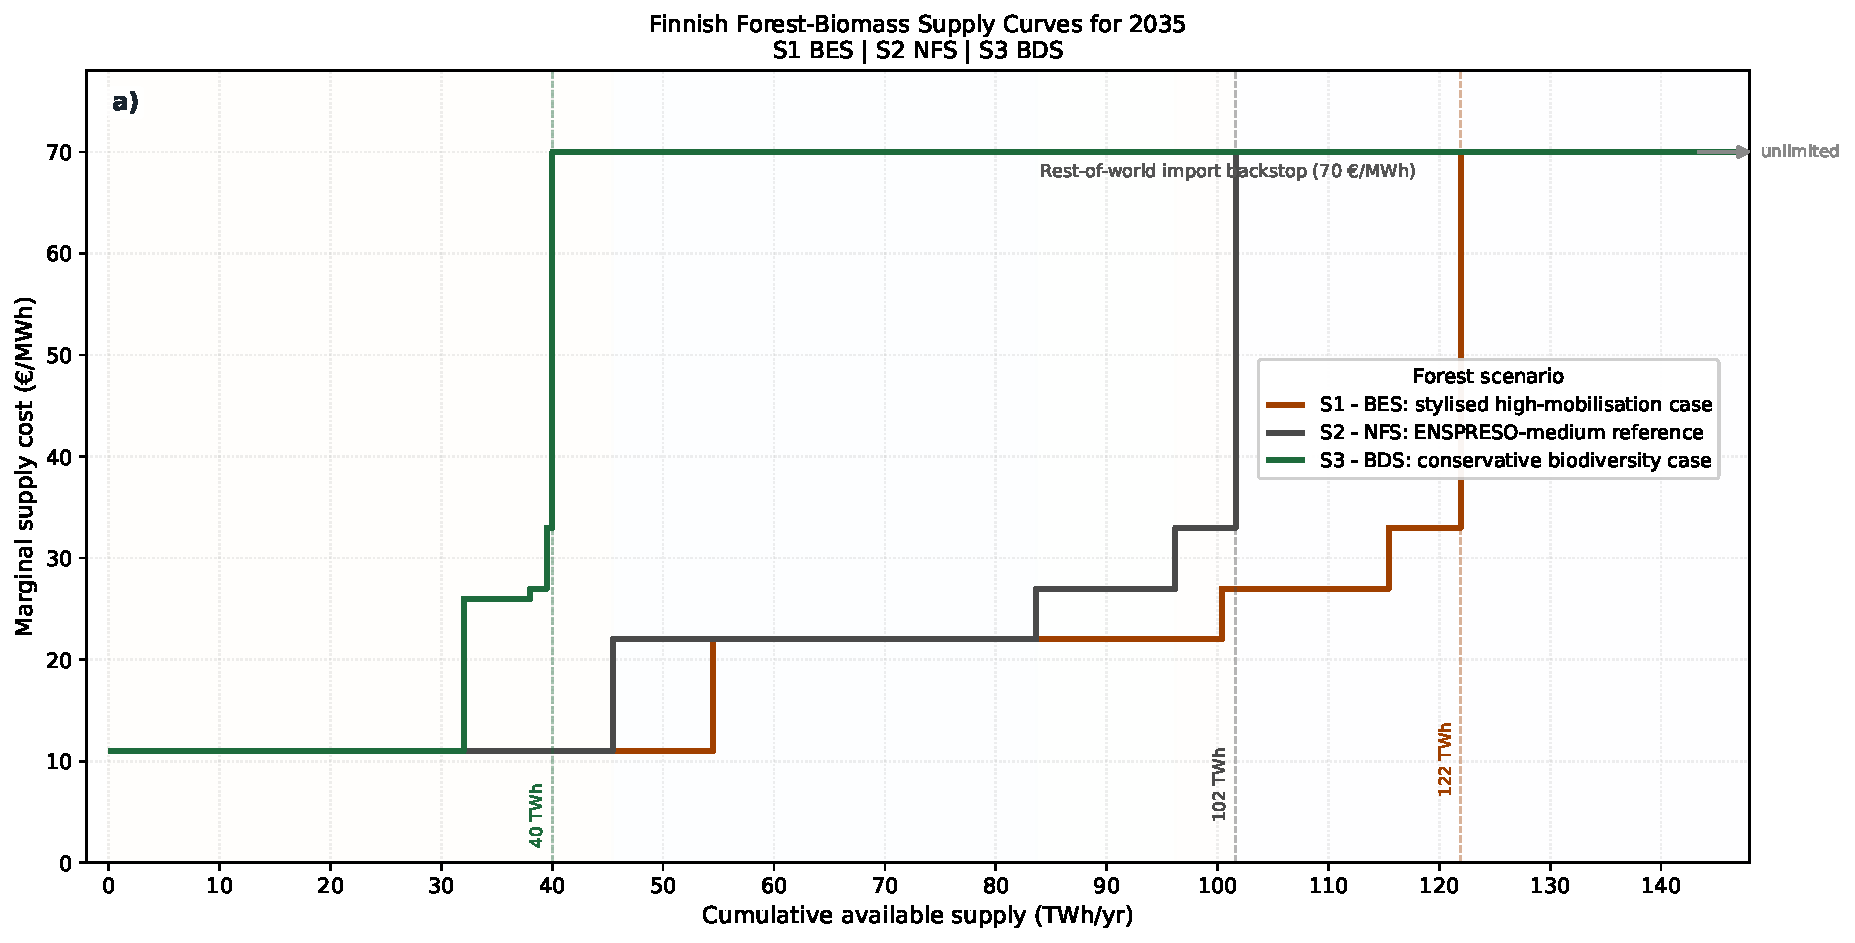
\includegraphics[width=0.98\linewidth]{biomass_supply_curves_fi_2035.pdf}
  \caption{Finnish forest-biomass supply curves used in the 2035 scenario matrix. The figure follows the Belgium logic of \citet{collaOptimalUseLignocellulosic2022} by presenting biomass as a stepwise cost ladder with step-specific embedded GHG, but simplifies the Finnish case into four domestic steps and one import backstop \citep{ruizENSPRESOOpenEU282019}. S1 is a stylised high-biomass sensitivity bound (+20\% above the ENSPRESO medium 2035 baseline), S2 the ENSPRESO-medium reference, and S3 a conservative biodiversity-constrained case revised against \citet{blattertSectoralPoliciesCause2022}, \citet{monkkonenEcologicallyEconomicallySustainable2024}, and recent Finnish national wood-energy statistics \citep{lukeWoodEnergy2024}.}
  \label{fig:fi_biomass_supply_curve}
\end{figure}

\paragraph{Interpretation and limitations of the first-stage ladder.}
Table~\ref{tab:fi_biomass_ladder} and Figure~\ref{fig:fi_biomass_supply_curve} represent an explicit first-stage calibration rather than a claim that every Finnish wood fraction has been fully characterised. Two limitations matter in particular. First, the step-specific GHG coefficients are simplifying supply-chain coefficients that preserve the relative logic of the Belgian framework, namely that more marginal or more distant biomass tends to be more carbon-intensive, but they are not a full reimplementation of the Belgium origin-by-quality RED~II matrix. Second, because the Belgian low-quality share constraint is not yet reintroduced, the Finnish first stage is stronger on transparent supply ranking than on physical feedstock-quality constraints. For the present paper, this keeps the focus on how domestic forest biomass availability changes across management narratives, but future work should strengthen the feedstock-quality treatment.

\paragraph{2035 forest scenario qualification and retained matrix.}
The retained forward-looking analysis uses a completed $3 \times 3$ scenario matrix. The forest dimension consists of S1/BES, S2/NFS, and S3/BDS. The policy dimension consists of an unconstrained case, a -95\% GHG case, and a -95\% GHG case with full nuclear phase-out. This final matrix excludes the earlier 80\% GHG column and the original optimistic S3-BDS value of 74.2~TWh. The completed runs show that the unconstrained 2035 system is already strongly decarbonised, whereas the conservative S3 case immediately saturates its 40~TWh ceiling under the -95\% target and therefore removes forest biomass as a flexible adjustment margin.

\paragraph{Boundary of the current paper.}
This paper reports the calibrated 2017 benchmark, the static 2035 forest-biomass ladder, and the completed forest-by-GHG scenario matrix. Disturbance shocks (windthrow, bark-beetle outbreaks, wildfire, salvage wood pulses, and dynamic price shocks) remain future work and are treated as the logical continuation of the present study rather than as implemented results.

\section{Results}
\label{sec:results}

\subsection{Finland 2017 Validation}

To establish model credibility before turning to forward-looking scenarios, the Finnish implementation of EnergyScope was calibrated against a historical baseline year. The final reference run is \texttt{20260323\_173930\_\_2017\_baseline} (\texttt{v37\_solar} in the run notes), solved with 12 typical days and \texttt{relax\_co2 = true} in order to avoid a non-physical forced-CCS artefact in the historical reproduction. The purpose of this benchmark is not to claim predictive validation of the future, but to test whether a constrained historical configuration can reproduce the known structure of the Finnish 2017 energy system with acceptable deviations.

Table~\ref{tab:fi_validation_2017} summarises the main indicators of the calibrated benchmark against the Finnish 2017 reference values. The main result is that the model reproduces the overall primary-energy balance, electricity mix, and net CO$_2$ emissions with high fidelity. All major primary-energy aggregates except solar remain within about $\pm 5\%$, electricity imports and CHP generation are also close to the statistical reference, and total net CO$_2$ emissions are reproduced almost exactly.

This agreement is also visible in Figure~\ref{fig:fi_validation_main}, which provides the two main graphical validation checks retained in the paper. The left panel shows that the model reproduces the dominant Finnish 2017 primary-energy pillars, especially biomass, oil, gas, coal and nuclear, without requiring large compensating errors across fuels. The right panel shows that the electricity balance is also captured at the right order of magnitude, with the main remaining deviation concentrated in gas-based generation rather than in the low-carbon backbone of nuclear, hydro and wind.

Two residual mismatches should nevertheless be discussed explicitly. First, district-heating production is overestimated by 43.4\%. This is not primarily a calibration failure but a structural aggregation artefact: in the present EnergyScope formulation, the district-heating share is applied to the full low-temperature heat pool, including industrial low-temperature demand, whereas Finnish statistics mainly report residential and service-sector network heat. Second, gas-fired electricity remains 36.7\% above the statistical reference because district-heating CHP in the model produces electricity as an unavoidable by-product when gas is routed through CHP technologies. These limitations do not invalidate the historical benchmark, but they define the clearest remaining structural aggregation issues.

\begin{table}[t]
  \centering
  \small
  \renewcommand{\arraystretch}{1.08}
  \begin{tabularx}{\linewidth}{llrrr}
    \toprule
    \textbf{Category} & \textbf{Indicator} & \textbf{Actual 2017} & \textbf{Model} & \textbf{Error} \\
    \midrule
    Primary energy & Biomass & 100.0 & 96.8 & -3.2\% \\
    Primary energy & Oil & 82.0 & 80.9 & -1.4\% \\
    Primary energy & Gas & 20.0 & 20.0 & 0.0\% \\
    Primary energy & Coal + peat & 35.0 & 35.0 & 0.0\% \\
    Primary energy & Nuclear & 65.0 & 65.1 & +0.1\% \\
    Primary energy & Hydro & 15.0 & 14.6 & -2.7\% \\
    Primary energy & Wind & 5.0 & 4.8 & -4.1\% \\
    Electricity & CHP & 20.73 & 20.49 & -1.2\% \\
    Electricity & Gas power & 3.2 & 4.37 & +36.7\% \\
    Electricity & Imports & 20.43 & 19.54 & -4.4\% \\
    Heat & District-heating production & 36.5 & 52.33 & +43.4\% \\
    Emissions & CO$_2$ & 41.2 & 41.25 & +0.1\% \\
    \bottomrule
  \end{tabularx}
  \caption{Main indicators of the calibrated Finland 2017 benchmark against the statistical reference system. Primary energy and electricity values are in TWh; CO$_2$ emissions in MtCO$_2$/y. Values are from run \texttt{20260323\_173930\_\_2017\_baseline}.}
  \label{tab:fi_validation_2017}
\end{table}

\begin{figure}[t]
  \centering
  \begin{minipage}{0.49\linewidth}
    \centering
    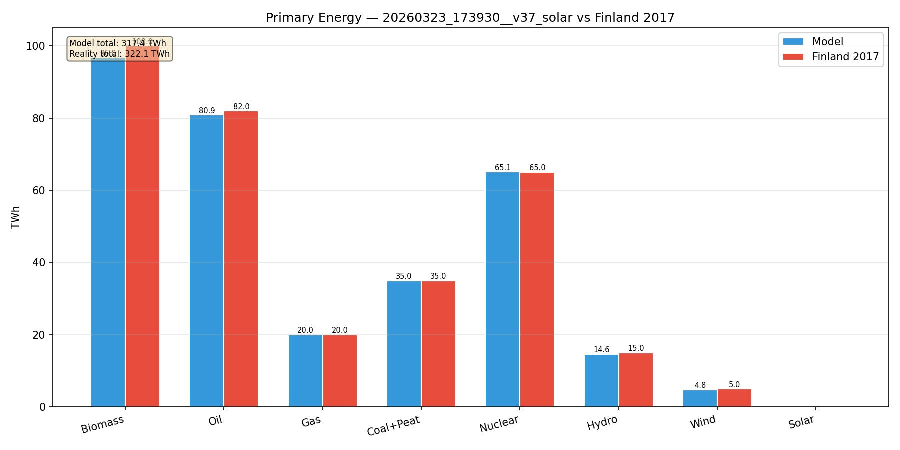
\includegraphics[width=\linewidth]{validation_2017_pe_comparison.pdf}
  \end{minipage}
  \hfill
  \begin{minipage}{0.49\linewidth}
    \centering
    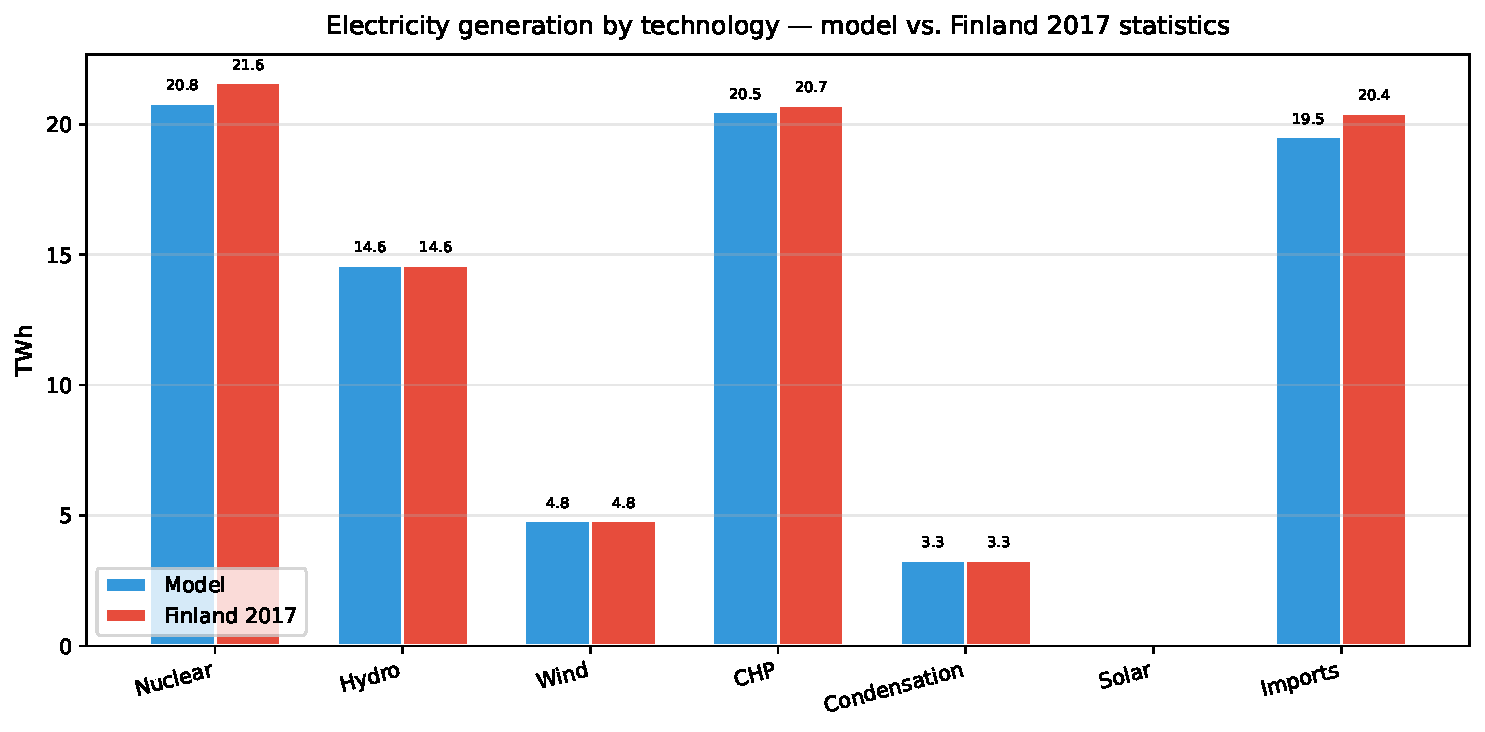
\includegraphics[width=\linewidth]{validation_2017_elec_comparison.pdf}
  \end{minipage}
  \caption{Main validation plots for the calibrated Finland 2017 benchmark. Left: primary-energy comparison between the model and Finnish 2017 statistics. Right: electricity-generation comparison for the same benchmark.}
  \label{fig:fi_validation_main}
\end{figure}

For the main text, the retained validation visuals are therefore limited to the primary-energy comparison, the electricity-generation comparison, and a structural Sankey view of the calibrated system. Figure~\ref{fig:fi_validation_sankey} complements Figure~\ref{fig:fi_validation_main} by showing that the calibrated benchmark is not only numerically close to Finnish statistics but also structurally coherent as an integrated energy system. In particular, the corrected heat-pump branch makes clear that low-temperature heat is produced from a combination of electricity and ambient heat, while the broader diagram highlights the expected roles of nuclear and hydro in electricity supply, lignocellulosic biomass in heat and CHP, and oil products in mobility and non-energy uses.

\begin{figure}[t]
  \centering
  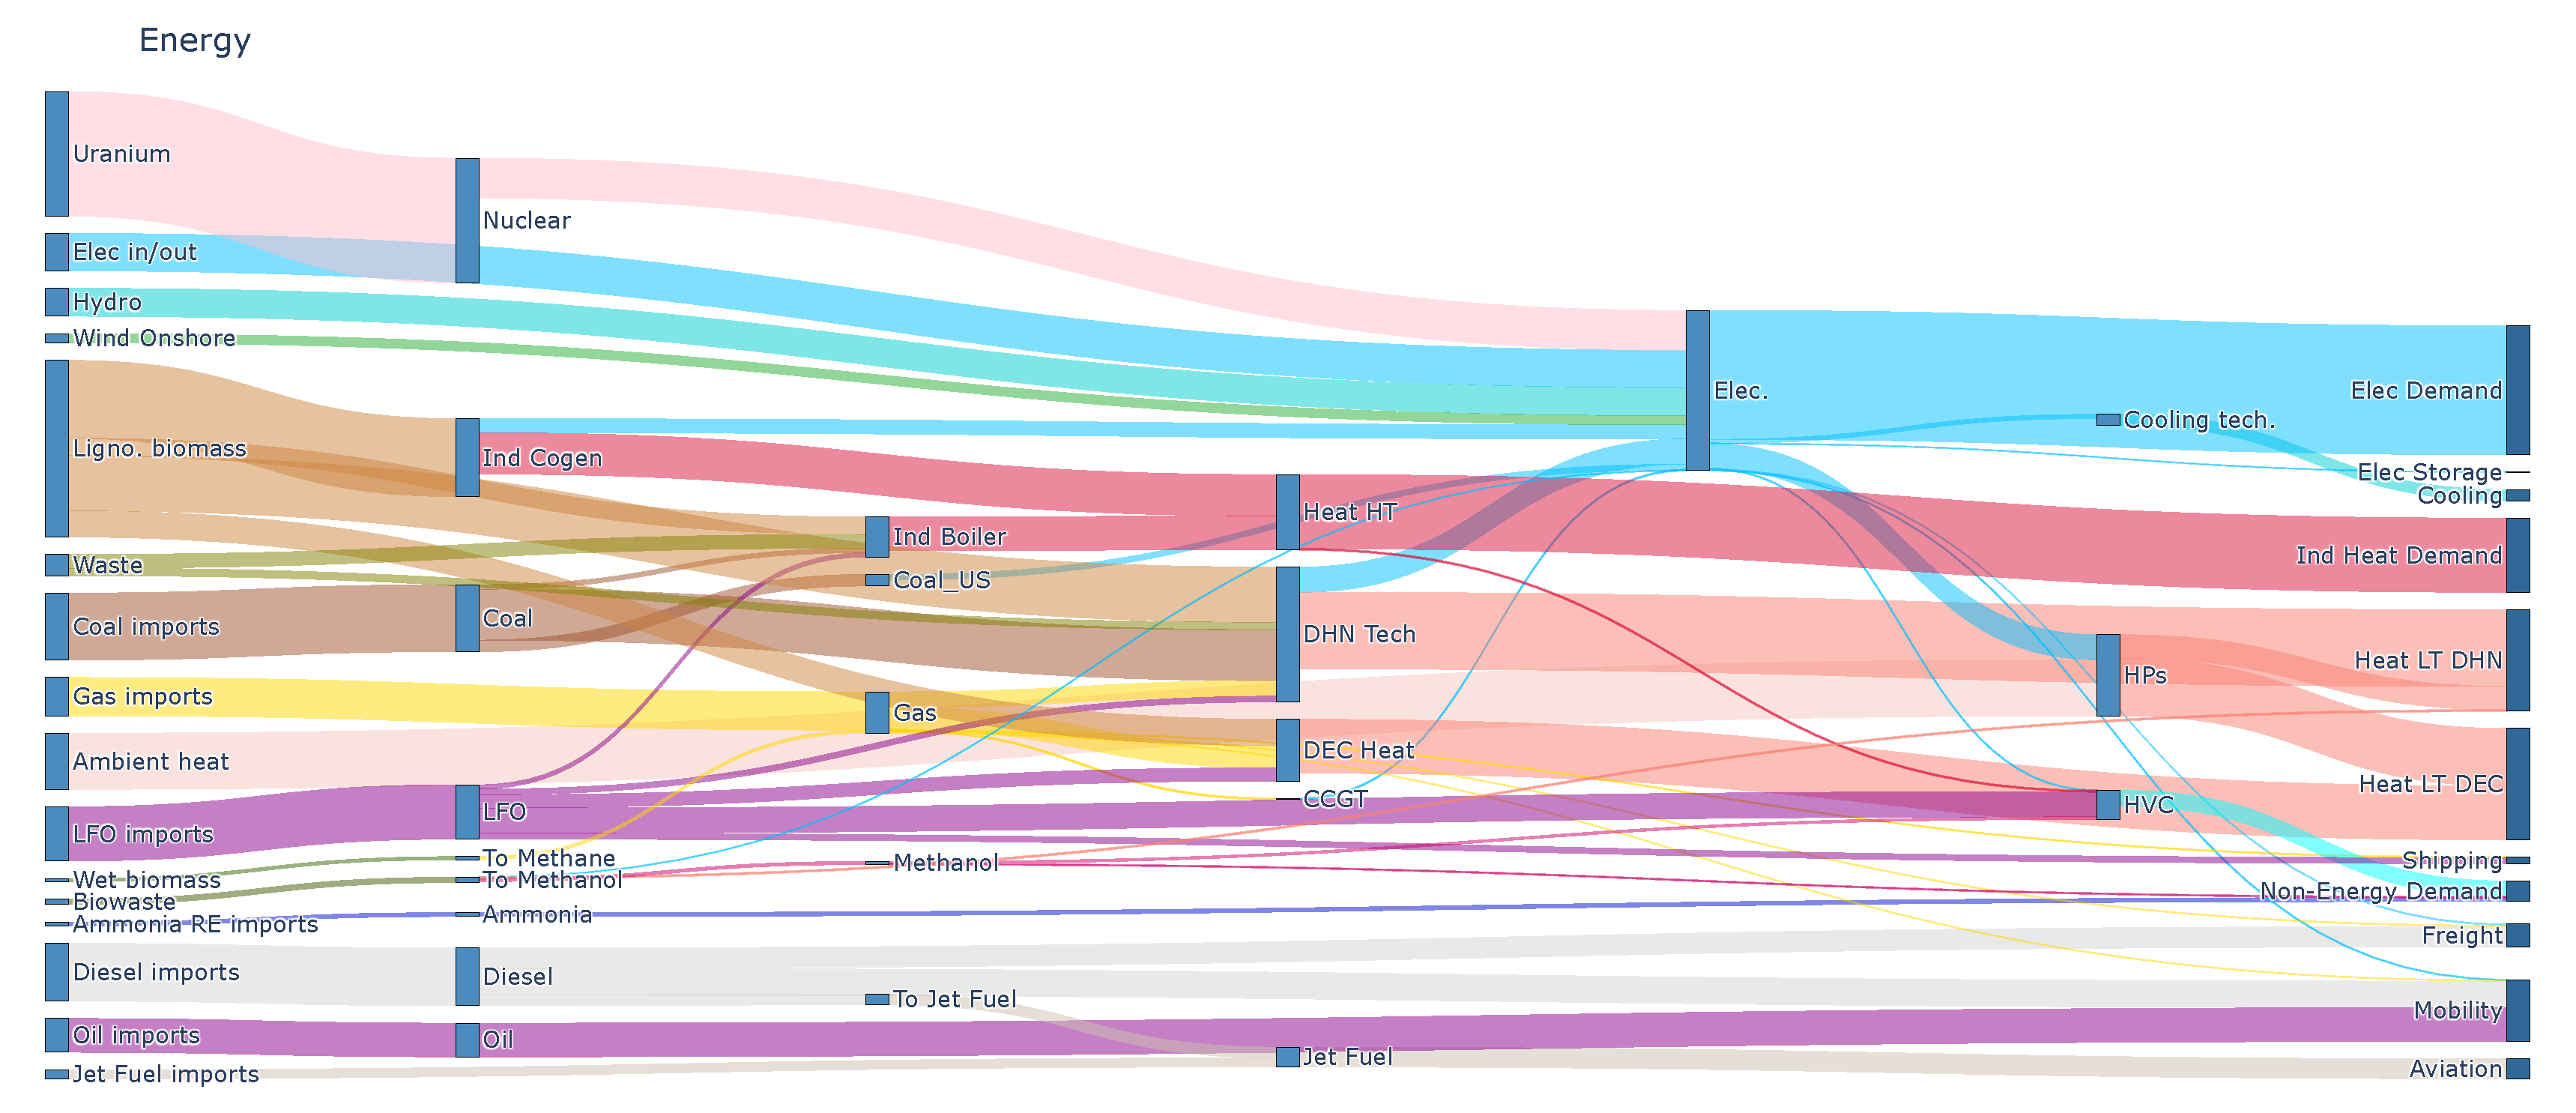
\includegraphics[width=\linewidth]{validation_2017_sankey.pdf}
  \caption{Structural Sankey view of the calibrated Finland 2017 benchmark. The corrected heat-pump node is balanced by both electricity and ambient heat inflows, avoiding the misleading appearance of net heat creation in the validation visualisation.}
  \label{fig:fi_validation_sankey}
\end{figure}

\subsection{Finland 2035 Results Under Forest and Emissions Scenarios}

The forward-looking analysis uses the completed $3 \times 3$ matrix crossing three forest-biomass supply narratives (S1/BES, S2/NFS, S3/BDS) with three policy configurations (unconstrained, -95\% GHG with nuclear, and -95\% GHG with full nuclear phase-out). Across the three forest cases, the unconstrained 2035 optimum already yields net CO$_2$ emissions between about 12.6 and 13.1~MtCO$_2$/y, corresponding to roughly 68--70\% reduction relative to 2017. The policy-relevant question is therefore not whether the unconstrained 2035 system decarbonises, but how the last part of the path toward a -95\% target changes when forest biomass becomes scarce and nuclear is removed.

Table~\ref{tab:fi_2035_matrix} summarises the main results of the retained scenario matrix. Three patterns deserve emphasis. First, the unconstrained cases are relatively close in annualised system cost, but they already differ in biomass use: S3/BDS is more constrained than S1 and S2 even without a climate target. A structural detail worth noting is that in all three unconstrained cases the model saturates exactly the first supply-ladder step (WOOD\_FI1, cheap industrial by-products) and draws nothing from the higher-cost domestic steps, indicating that the 2035 Finnish energy demand without a climate target can be met entirely from the cheapest biomass fractions; the supply-curve design therefore matters primarily under the stringent GHG constraint. Second, the -95\% case with nuclear fully saturates the conservative S3 ceiling while leaving headroom in S1 and S2. Third, removing nuclear substantially increases biomass demand in S1 and S2 (from 74.2~TWh to 100.4~TWh in S1, and to 96.2~TWh in S2), yet the additional system cost is surprisingly small: only 0.02 and 0.10~bn~EUR/y respectively, because the additional wood is available at the intermediate steps of an unconstrained supply ladder. By contrast, S3 cannot expand further because its 40~TWh domestic ceiling is already binding, making the nuclear phase-out more costly (0.34~bn~EUR/y additional). In other words, S3 does not make deep decarbonisation infeasible in the optimiser, but it removes forest biomass as a flexible adjustment margin and therefore becomes the highest-cost configuration, with a sensitivity to nuclear availability roughly three times greater than in S1.

These system-level shifts are easier to read in Figure~\ref{fig:fi_2035_energy_matrix}. The top row shows that the main transition from the unconstrained cases to the -95\% cases is not a simple linear reduction in fossil use, but a reconfiguration of the entire primary-energy mix around electricity, nuclear availability, and scarce biomass. The bottom row shows that the forest-wood ladder is only partially mobilised in the unconstrained cases, whereas the stringent climate cases move rapidly up the ladder and, in S3/BDS, hit the domestic ceiling. This is the key result of the scenario exercise: biodiversity-constrained forest supply does not prevent deep decarbonisation in the model, but it removes cheap domestic biomass as an adjustment margin precisely when the climate constraint becomes stringent.

Figure~\ref{fig:fi_2035_biomass_allocation} adds the end-use interpretation behind that aggregate picture. In S1/BES and S2/NFS, the no-nuclear variants redirect more biomass toward the hardest-to-abate services, indicating that biomass is treated as a strategic balancing resource once zero-carbon baseload flexibility declines. By contrast, S3/BDS cannot respond to the same pressure by expanding forest harvest, so the model is forced to reallocate scarce biomass more selectively and lean more heavily on non-biomass substitutions elsewhere in the system. The policy implication is that the debate is not only about the total quantity of forest biomass available, but also about which end uses receive priority when both climate ambition and forest constraints tighten.

\begin{table}[t]
  \centering
  \small
  \renewcommand{\arraystretch}{1.08}
  \begin{tabularx}{\linewidth}{llrrr}
    \toprule
    \textbf{Forest scenario} & \textbf{Policy case} & \textbf{Cost} & \textbf{CO$_2$ net} & \textbf{Forest wood used} \\
    \midrule
    S1/BES & Unconstrained & 22.40 bnEUR/y & 13.02 Mt/y & 54.5 TWh \\
    S1/BES & -95\% GHG (with nuclear) & 22.92 bnEUR/y & 2.06 Mt/y & 74.2 TWh \\
    S1/BES & -95\% GHG (nuclear phase-out) & 22.94 bnEUR/y & 2.06 Mt/y & 100.4 TWh \\
    S2/NFS & Unconstrained & 22.46 bnEUR/y & 12.57 Mt/y & 45.4 TWh \\
    S2/NFS & -95\% GHG (with nuclear) & 23.02 bnEUR/y & 2.06 Mt/y & 74.2 TWh \\
    S2/NFS & -95\% GHG (nuclear phase-out) & 23.12 bnEUR/y & 2.06 Mt/y & 96.2 TWh \\
    S3/BDS & Unconstrained & 22.62 bnEUR/y & 13.10 Mt/y & 32.0 TWh \\
    S3/BDS & -95\% GHG (with nuclear) & 23.56 bnEUR/y & 2.06 Mt/y & 40.0 TWh \\
    S3/BDS & -95\% GHG (nuclear phase-out) & 23.90 bnEUR/y & 2.06 Mt/y & 40.0 TWh \\
    \bottomrule
  \end{tabularx}
  \caption{Summary of the retained Finland 2035 forest-biomass scenario matrix. Forest-wood use sums the Finnish forest-biomass ladder resources only.}
  \label{tab:fi_2035_matrix}
\end{table}

\begin{figure}[t]
  \centering
  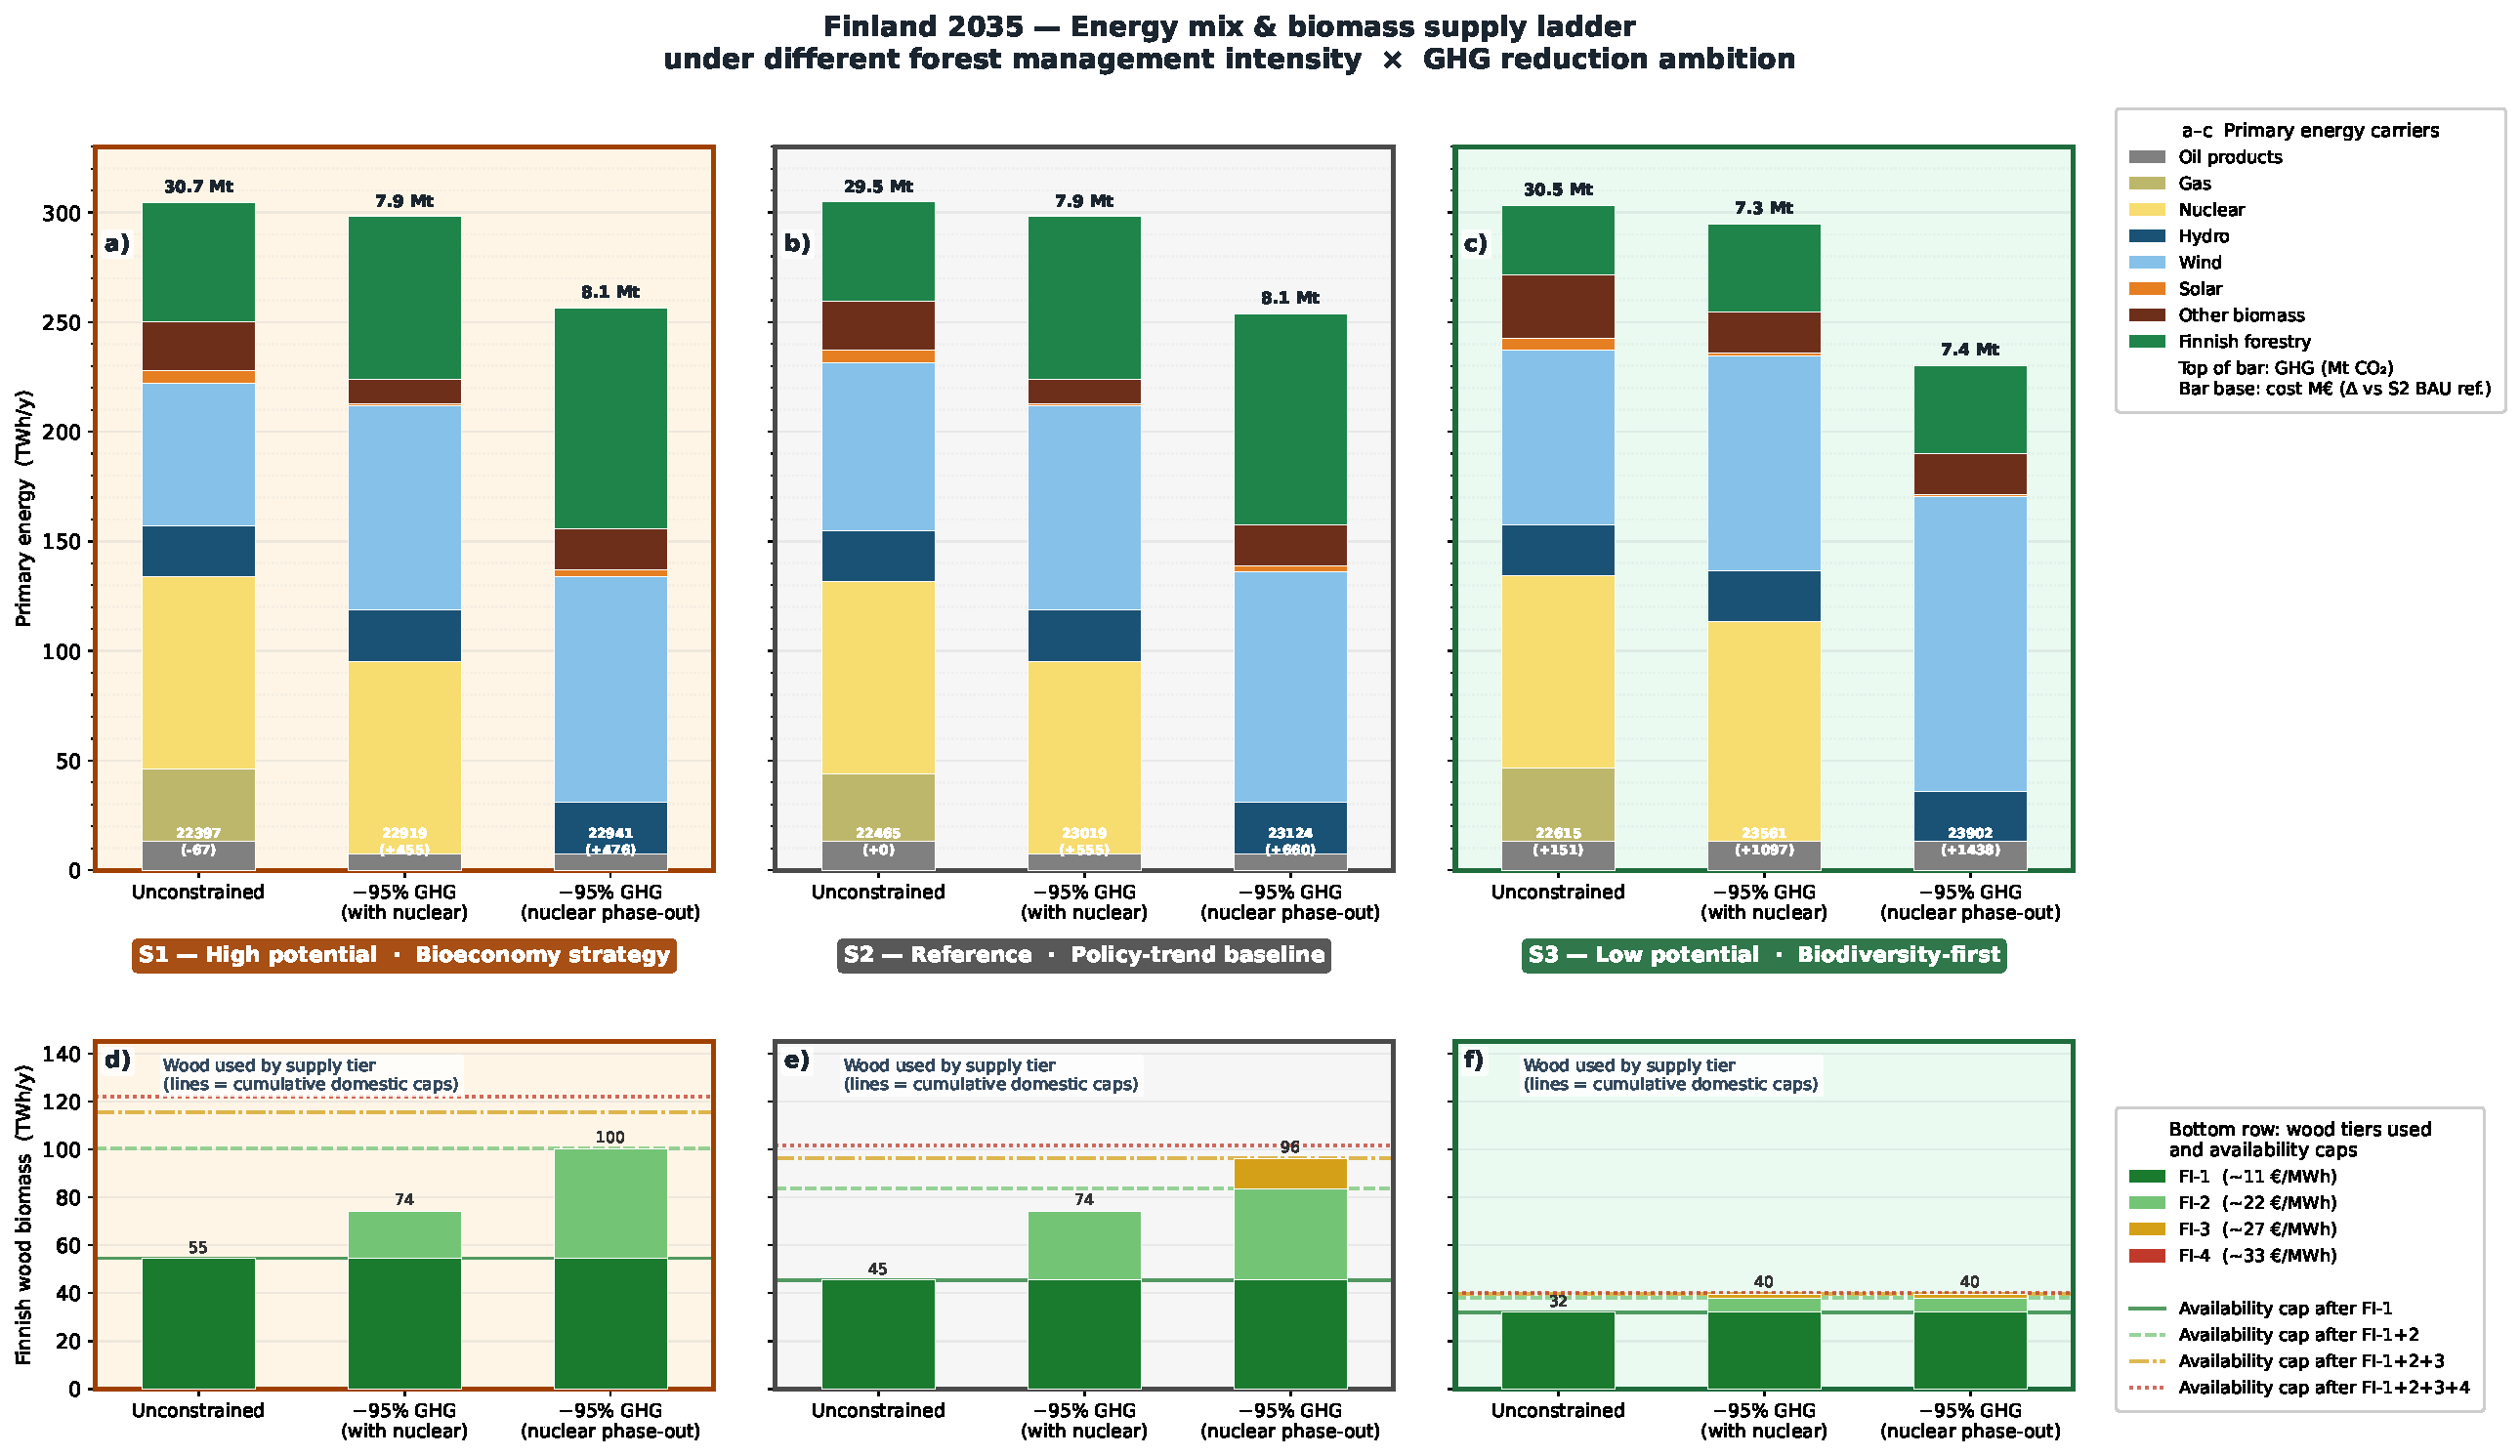
\includegraphics[width=\linewidth]{forest_scenarios_2035_energy_matrix.pdf}
  \caption{Finland 2035 scenario matrix across three forest-management cases and three GHG configurations. The top row shows the primary-energy mix, while the bottom row shows the use of the Finnish forest-wood supply ladder. The unconstrained cases already reach roughly a 70\% reduction versus 2017, while the biodiversity-constrained S3 case is distinguished by early saturation of the domestic wood ceiling under the -95\% target.}
  \label{fig:fi_2035_energy_matrix}
\end{figure}

\begin{figure}[t]
  \centering
  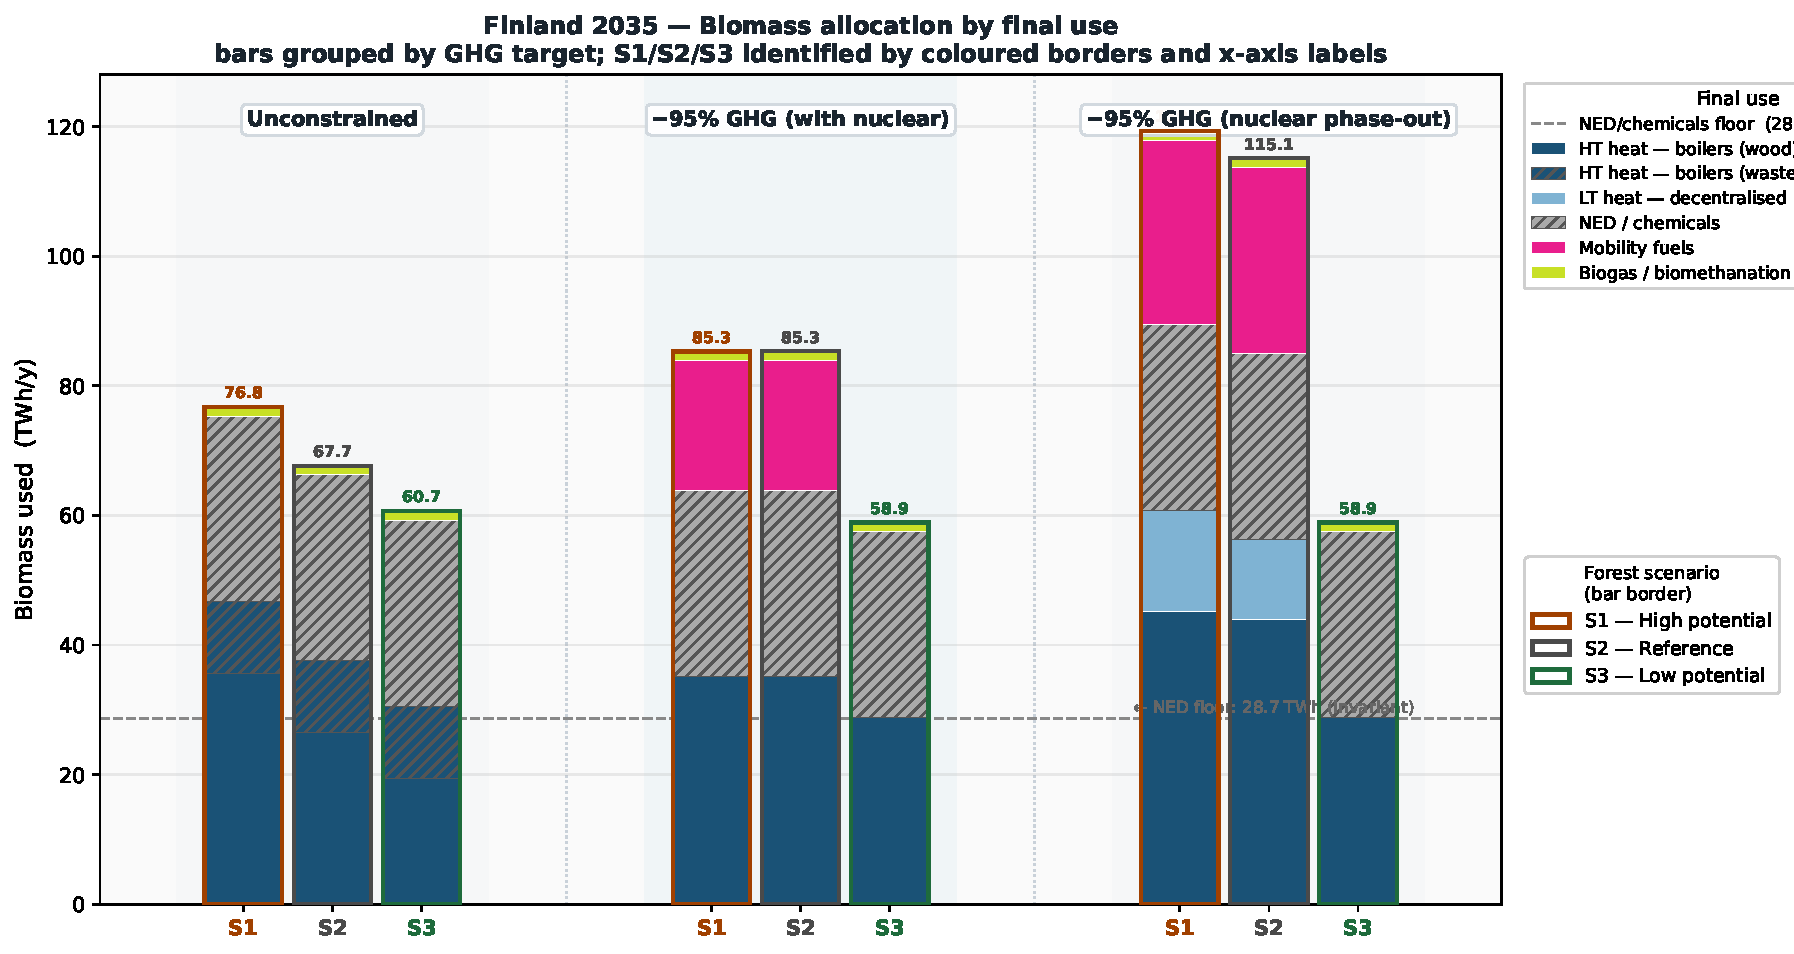
\includegraphics[width=\linewidth]{forest_scenarios_2035_biomass_allocation.pdf}
  \caption{Biomass allocation by final use in Finland 2035. The figure highlights how the no-nuclear cases increase pressure on biomass in S1 and S2, whereas S3/BDS remains capped by its conservative forest-biomass ceiling and therefore relies more heavily on non-biomass adjustments elsewhere in the system.}
  \label{fig:fi_2035_biomass_allocation}
\end{figure}

\subsection{Next steps: disturbance shocks and dynamic biomass supply}

The present paper deliberately stops at static 2035 management scenarios. The next stage of the research is to couple the Finnish forest simulator used by the Jyvaskyla/LUKE team with the FLAM and PICUS disturbance modules developed in the ForestNavigator framework, so that annual biomass supply curves can respond to wildfire risk, bark-beetle outbreaks, windthrow, salvageable calamity wood, and the subsequent reduction in standing stock \citep{venalainenClimateChangeInduces2020,hlasnyDevastatingOutbreakBark2021,tothImpactsCalamityLogging2020}. In energy-system terms, this would extend the current forest scenarios from fixed 2035 ladders to time-varying biomass availability and cost trajectories under contrasting management regimes and climate pathways.

The concept-note design is not simply a lower biomass ceiling. It is intended to capture three mechanisms that are absent from the current paper: a short-lived calamity-wood pulse after a disturbance event, quality and marginal-cost changes for salvage biomass, and a medium-term decline in future harvestable stock after damaged cohorts are depleted \citep{tothImpactsCalamityLogging2020,reckaRoleBiomassDecarbonisation2023}. Methodologically, the proposed extension uses a pre-shock 2030 EnergyScope snapshot, followed by a post-shock snapshot with limited re-optimisation in order to reflect realistic investment lead times for biomass CHP, DHN extensions, and other inherited infrastructure. The disturbance module is therefore presented as the logical next research phase built on the present article: the current paper establishes the calibrated national baseline and the static forest-scenario framework, while the coupled forest-disturbance workflow would add dynamic timing, quality, and price effects on top of that validated base.

\section{Conclusion}
\label{sec:conclusion}

This paper develops a first national EnergyScope TD application for Finland centred on the role of forest biomass in a 2035 transition setting. By translating contested forest-management narratives into explicit biomass supply curves, it links the Finnish forest-policy debate to whole-energy-system optimisation. The calibrated 2017 benchmark shows that the model can reproduce the main Finnish primary-energy aggregates, electricity balance, and net CO$_2$ emissions with high fidelity, while keeping the remaining structural mismatches transparent, especially for district heating and gas-related CHP co-production. This validation step is essential because it establishes that the Finnish implementation is sufficiently credible for scenario exploration before moving to forward-looking policy questions.

For the 2035 scenario matrix, the central result is not that biodiversity-constrained forest management makes deep decarbonisation impossible, but that it removes forest biomass as a low-cost adjustment margin exactly when climate ambition becomes stringent. The unconstrained 2035 cases are already strongly decarbonised, whereas the -95\% cases reveal much sharper competition for biomass, particularly when nuclear is removed. S1/BES and S2/NFS retain some flexibility to expand forest-wood use, but S3/BDS saturates its conservative 40~TWh ceiling and becomes the highest-cost configuration. The paper therefore shows that forest-biomass assumptions are not a secondary sensitivity: they materially shape the cost and allocation logic of deep decarbonisation in Finland. The next research step is to extend this validated static framework toward disturbance-driven annual biomass supply trajectories, so that wind, beetle, and wildfire shocks can be studied within the same energy-system optimisation framework.





\bibliographystyle{plainnat}
\bibliography{references}

\end{document}